\documentclass[xetex,10pt,mathserif]{beamer}

\usetheme{Boadilla}
\usecolortheme{seahorse}

\usefonttheme{professionalfonts}
\usepackage{fontspec}
\usepackage{xunicode}
\usepackage{xltxtra}
\setmainfont[Ligatures={Common,TeX}, Scale=0.95]{Myriad Pro}
\setsansfont[Ligatures={Common,TeX}, Scale=0.95]{Myriad Pro}

\usepackage{media9}
\usepackage{grfext}\PrependGraphicsExtensions*{.png,.PNG}


%%
\usepackage{tabularx}
\usepackage{mathtools}
\usepackage{xspace}
\usepackage{makecell}
\usepackage{msthpres}
\usepackage{pdfpages} 
%%

\usepackage{tikz}
\usetikzlibrary{arrows,positioning,shapes,fit}
\usepackage{pgfplots}
\usepgfplotslibrary{fillbetween,colormaps}
\newlength\figureheight
\newlength\figurewidth

% presentation stuff
\newcommand{\sig}[2]{%
\begin{tabular}{r}
#1\\[-0.7em]
{\tiny \color{darkgray}\it #2\hspace{0.5em}}
\end{tabular}}

\newcommand{\qauth}[1]{{\footnotesize\par\normalfont\hfill---\ \emph{#1}\par}}

\newcommand{\qcite}[1]{{\small\color{gray}[#1]}}

% math stuff
\newcommand{\defeq}{\vcentcolon=}
\newcommand{\LLC}{$L$-Lipschitz continuous}
\newcommand{\Reps}{R_{\epsilon}}
\newcommand{\Rbeps}{\bar{R}_{\epsilon}}
\newcommand{\Ro}{R_{0}}
\newcommand{\Rbo}{\bar{R}_{0}}
\newcommand{\xb}{\hat{\*x}}
\newcommand{\smid}{\ \middle\vert\ }
\newcommand{\bigsmid}{\ \big\vert\ }
\newcommand{\setdef}[2]{\left\{ #1 \smid #2 \right\}}
\newcommand{\bigsetdef}[2]{\big\{ #1 \bigsmid #2 \big\}}

\usepackage{xspace}
\newcommand{\algo}{{\sc\textsf{SafeOpt}}\xspace}
\newcommand{\gpucb}{{\sc\textsf{GP-UCB}}\xspace}
\newcommand{\localucb}{{\sc\textsf{Safe-UCB}}\xspace}

% Colored sets
\newcommand{\cst}{{\color{cyan!70!black}$S_t$}\xspace}
\newcommand{\ccst}{{\color{cyan!70!black}S_t}\xspace}
\newcommand{\cgt}{{\color{lime!70!black}$G_t$}\xspace}
\newcommand{\ccgt}{{\color{lime!70!black}G_t}\xspace}
\newcommand{\cmt}{{\color{orange!70!black}$M_t$}\xspace}
\newcommand{\ccmt}{{\color{orange!70!black}M_t}\xspace}
\newcommand{\crbo}{{\color{magenta!70!black}$\Rbo(S_0)$}\xspace}
\newcommand{\crbeps}{{\color{magenta!70!black}$\Rbeps(S_0)$}\xspace}
\newcommand{\ccrbeps}{{\color{magenta!70!black}\Rbeps(S_0)}\xspace}

\title[Non-monotone Adaptive Submodular Maximization]
{Non-monotone Adaptive Submodular Maximization}

\author[Alkis Gotovos]{
\vspace{1in}
\normalsize
\parbox{1in}{Alkis Gotovos\\{\footnotesize ETH Zurich}}\and
\parbox{1in}{Amin Karbasi\\{\footnotesize Yale University}}\and
\parbox{1in}{Andreas Krause\\{\footnotesize ETH Zurich}}
}

\date[May 4, 2015]{
\begin{center}
{\normalsize
ICML '15
}
\end{center}
}

\begin{document}

\setbeamercolor{background canvas}{bg=}

\includepdf[pages={1}]{title.pdf}

\begin{frame}{Birdwatching}
\centering
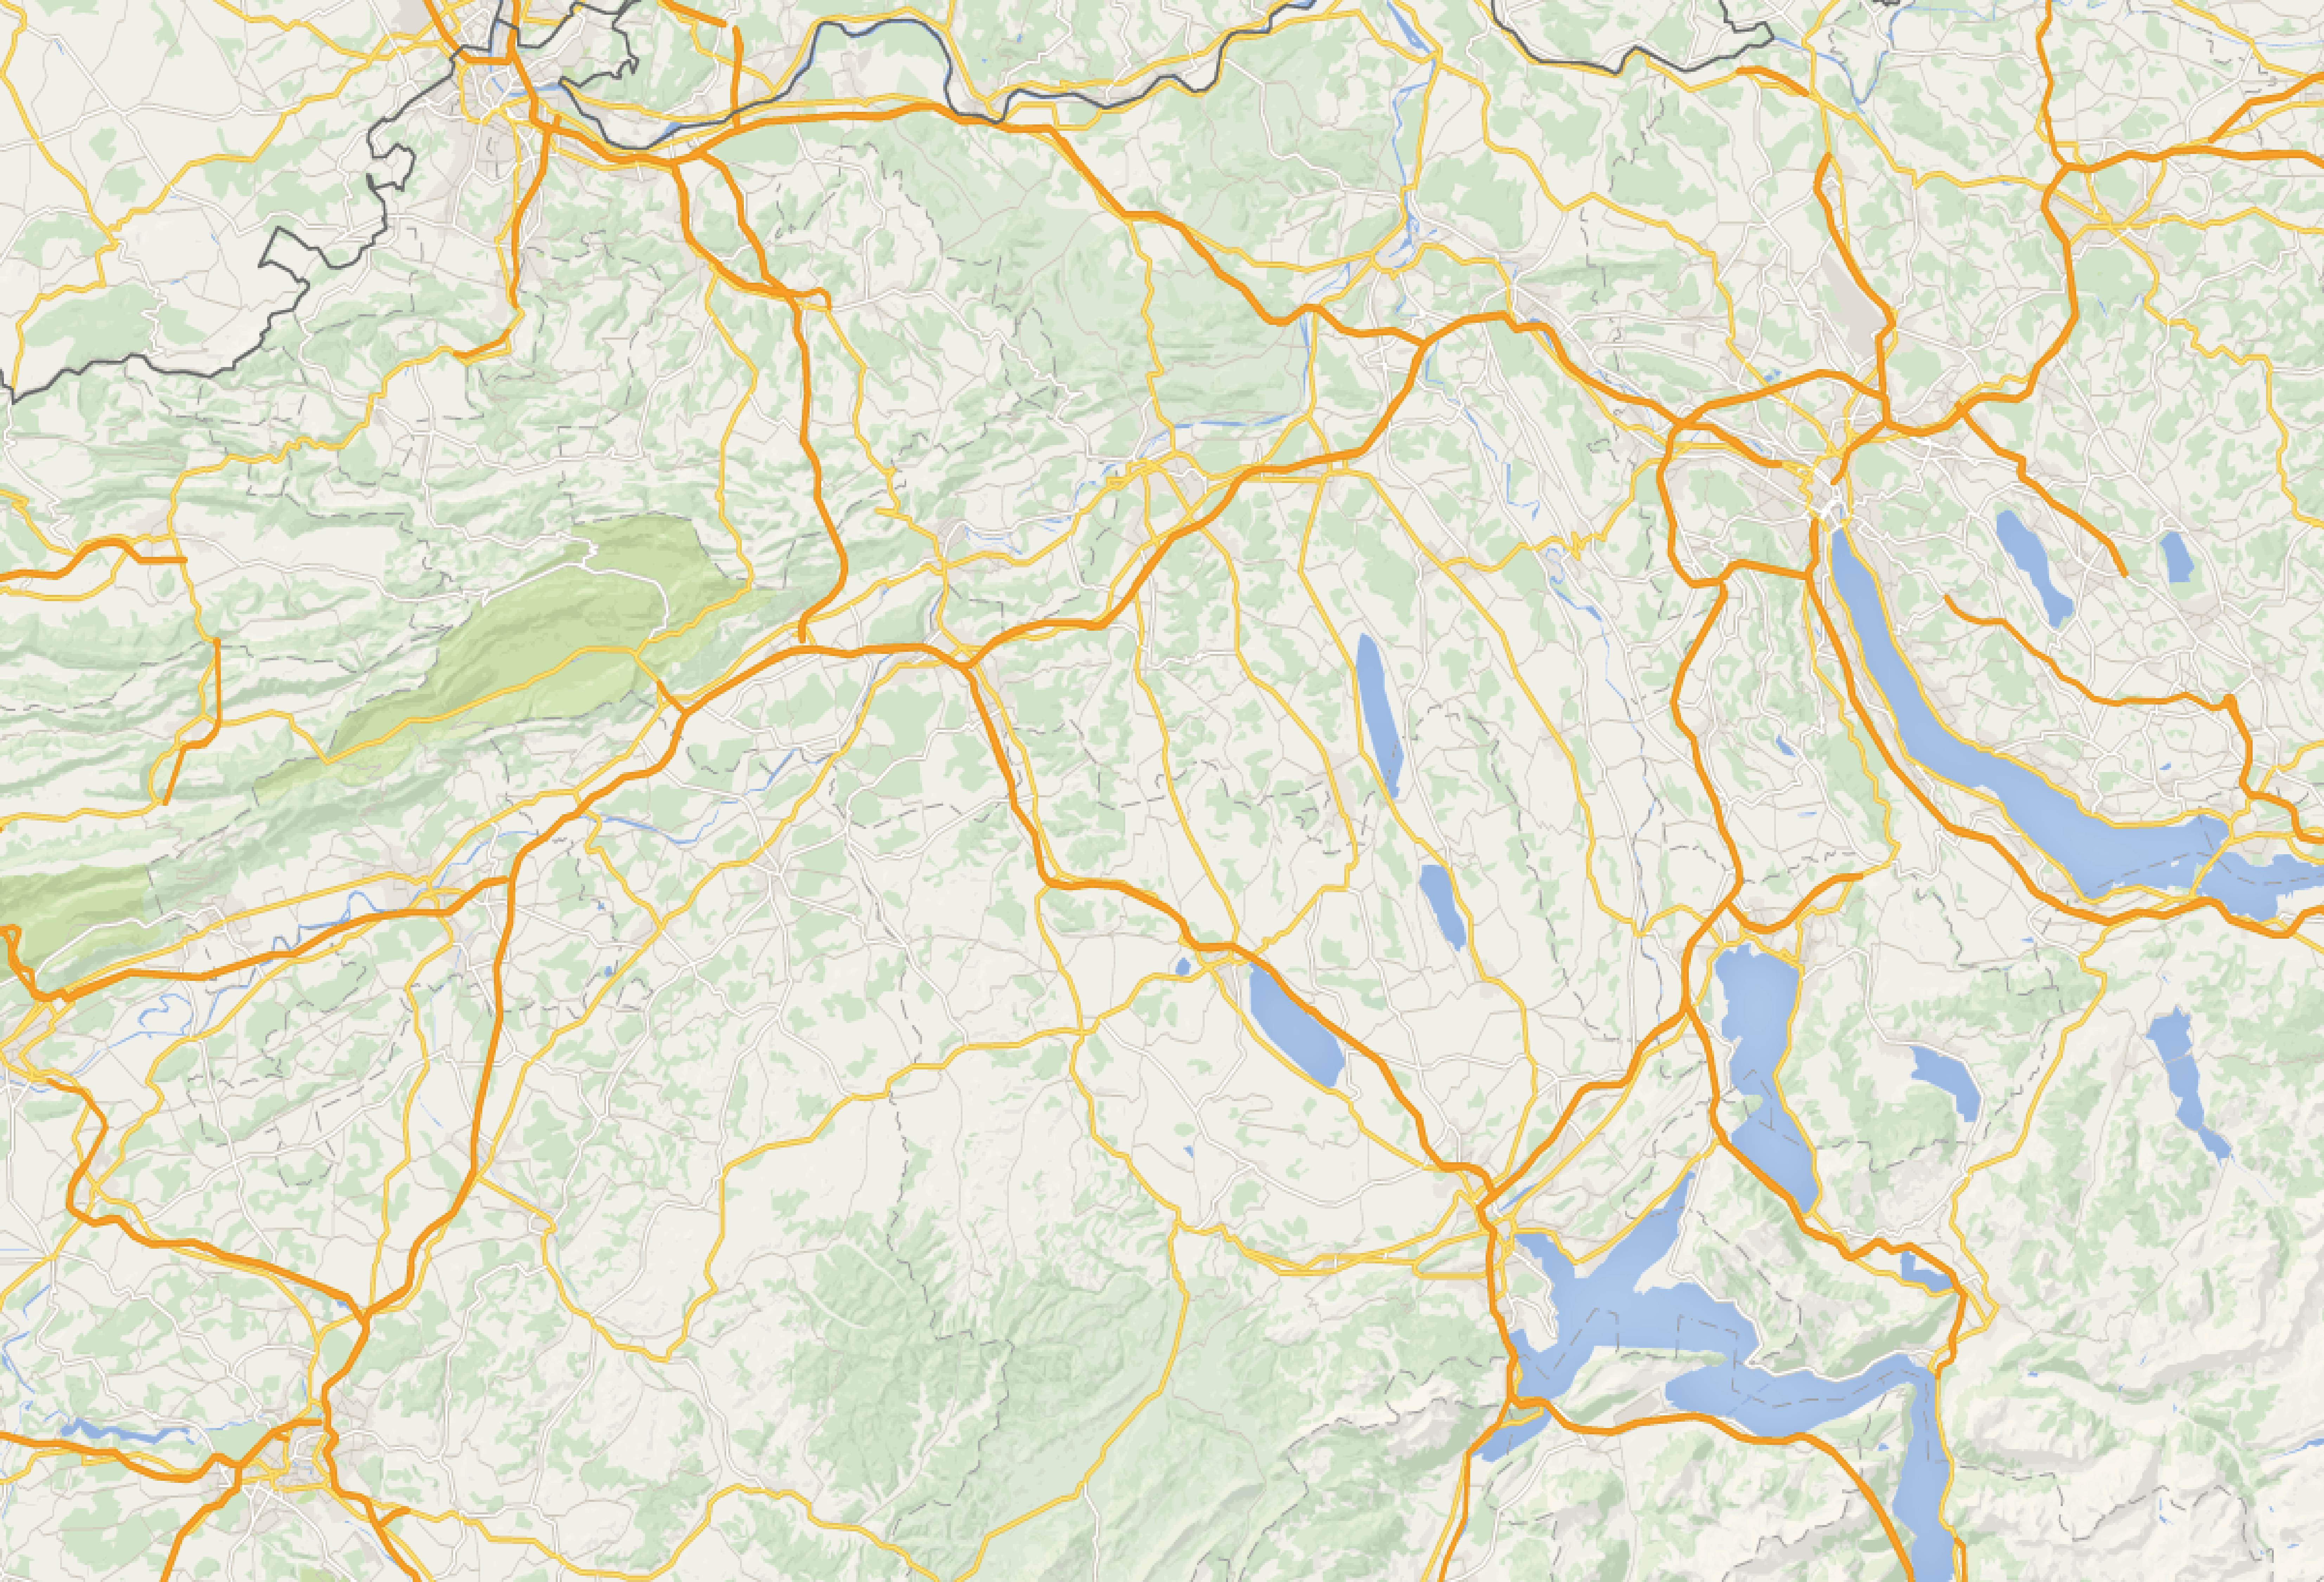
\includegraphics[width=4.75in]{figures/map.pdf}
\end{frame}

\begin{frame}{Birdwatching}
\centering
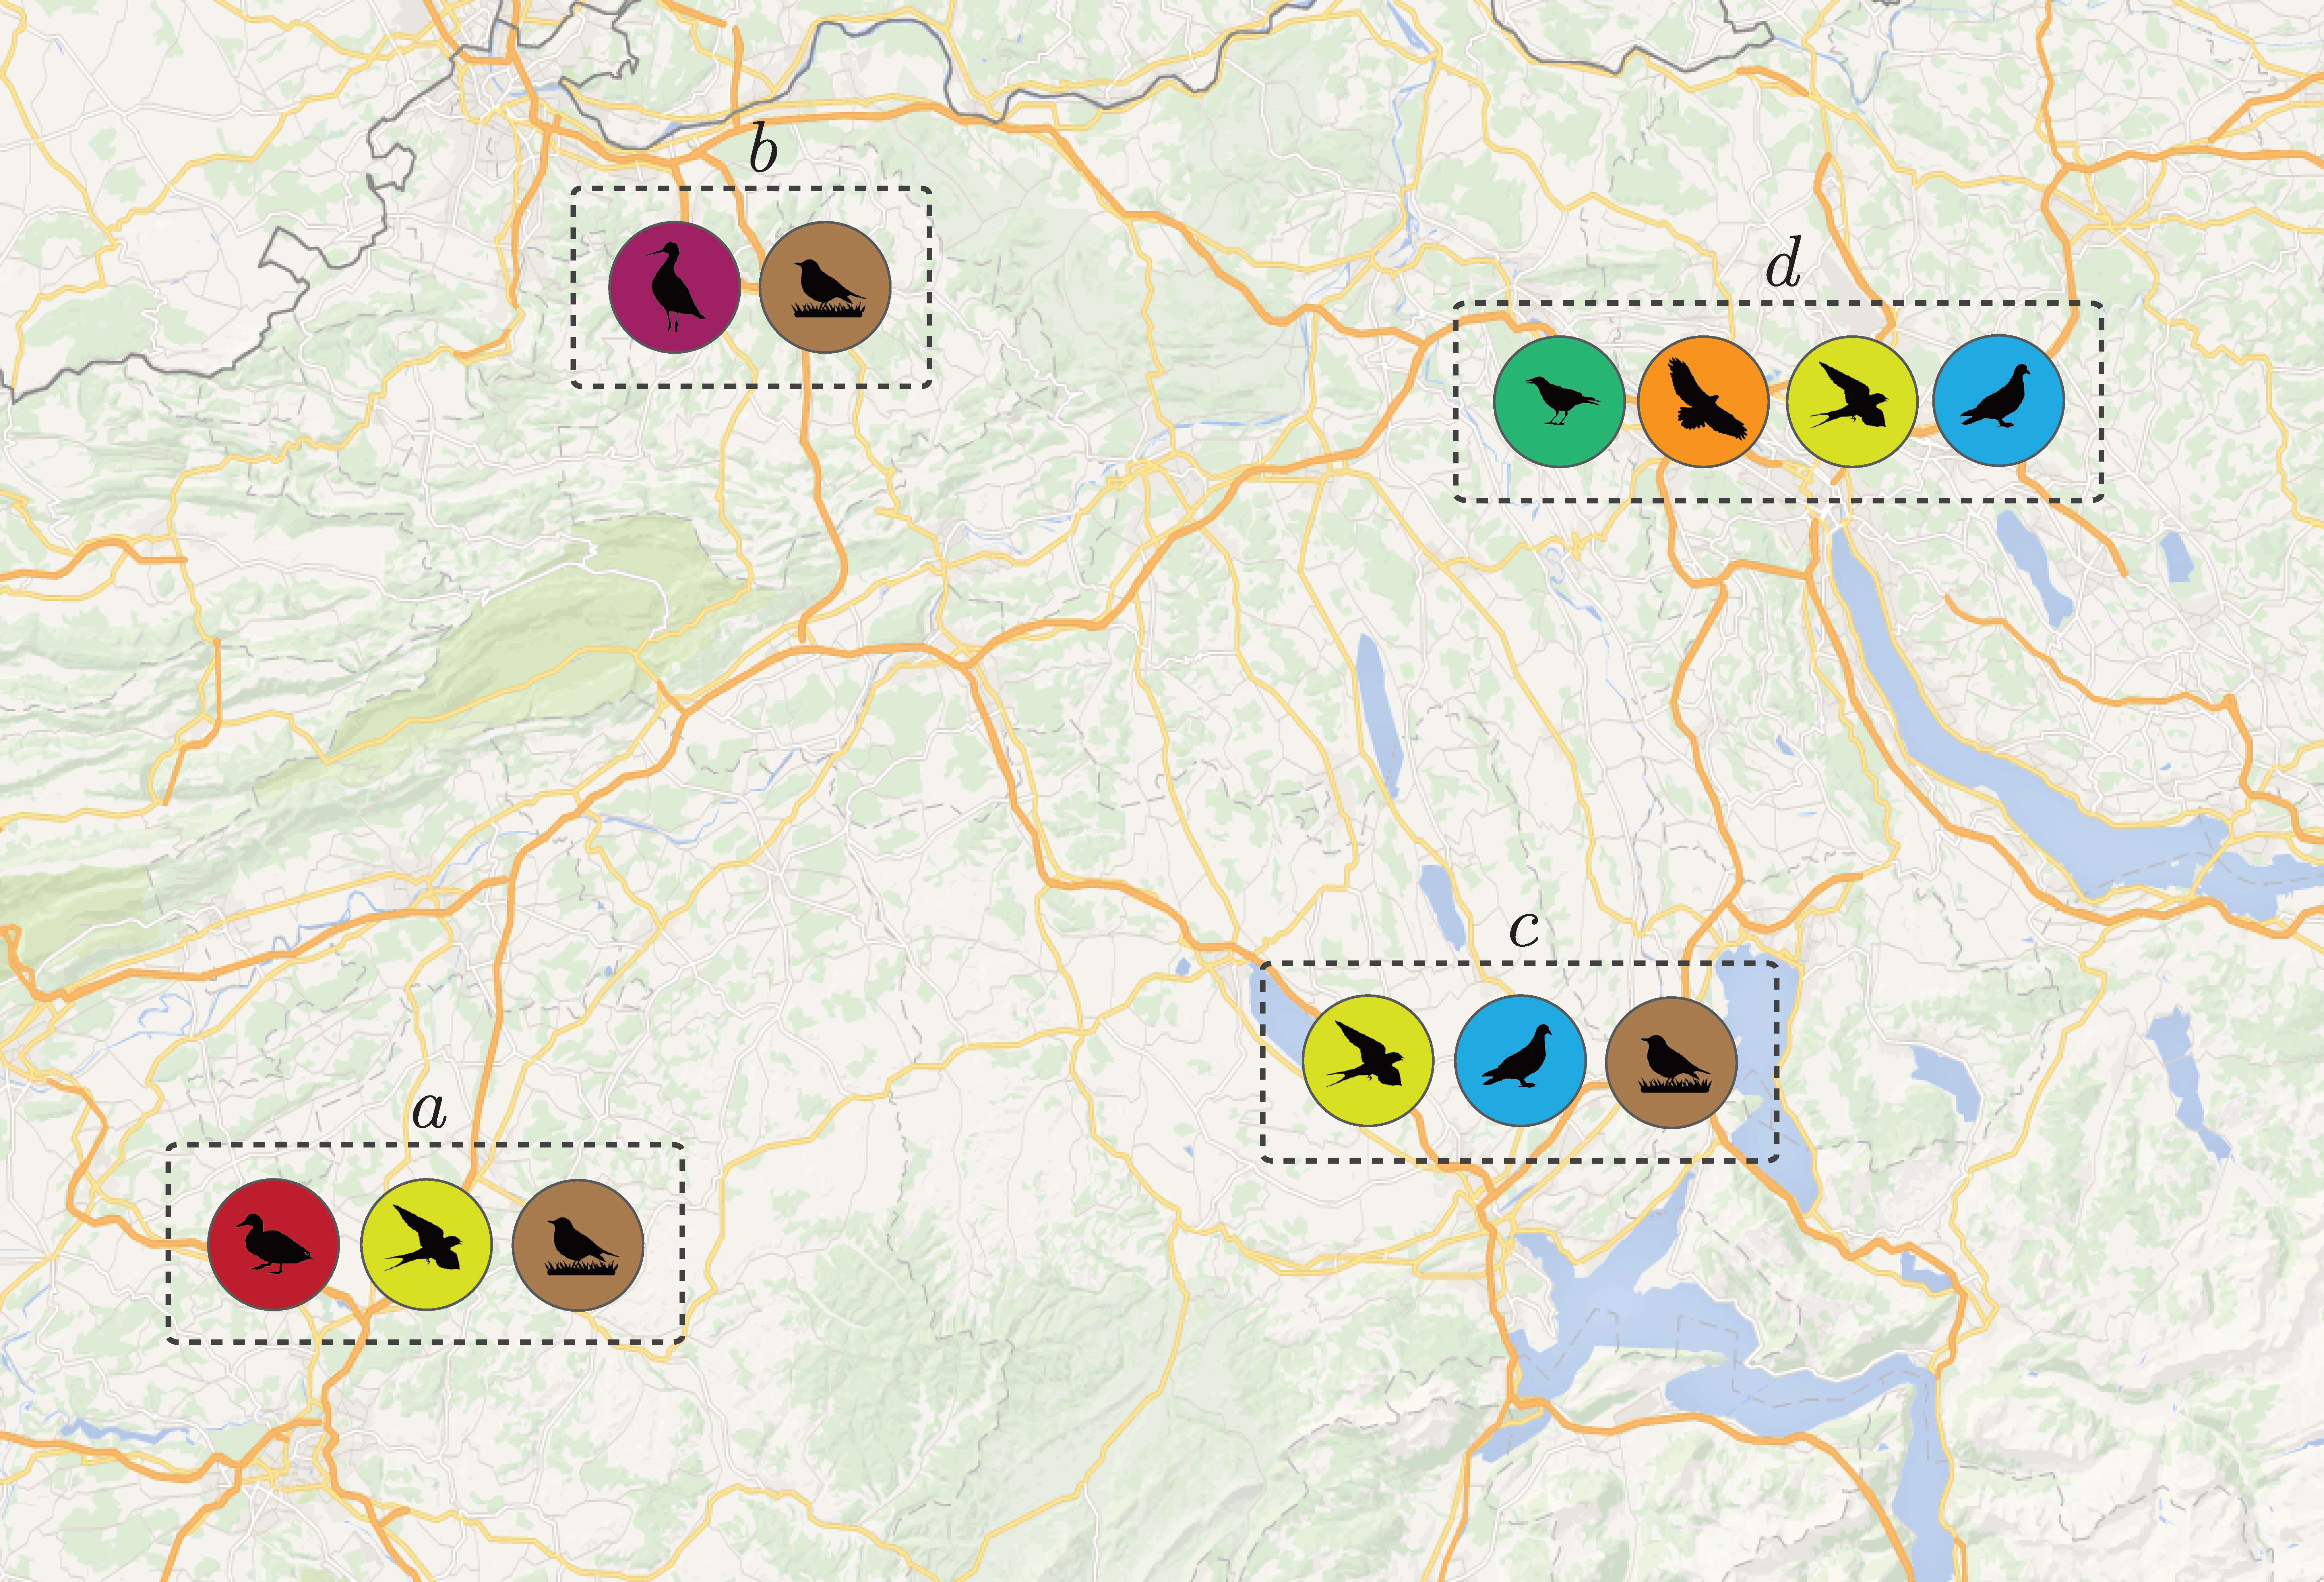
\includegraphics[width=4.75in]{figures/intro_1.pdf}
\end{frame}

\begin{frame}{Birdwatching}
\centering
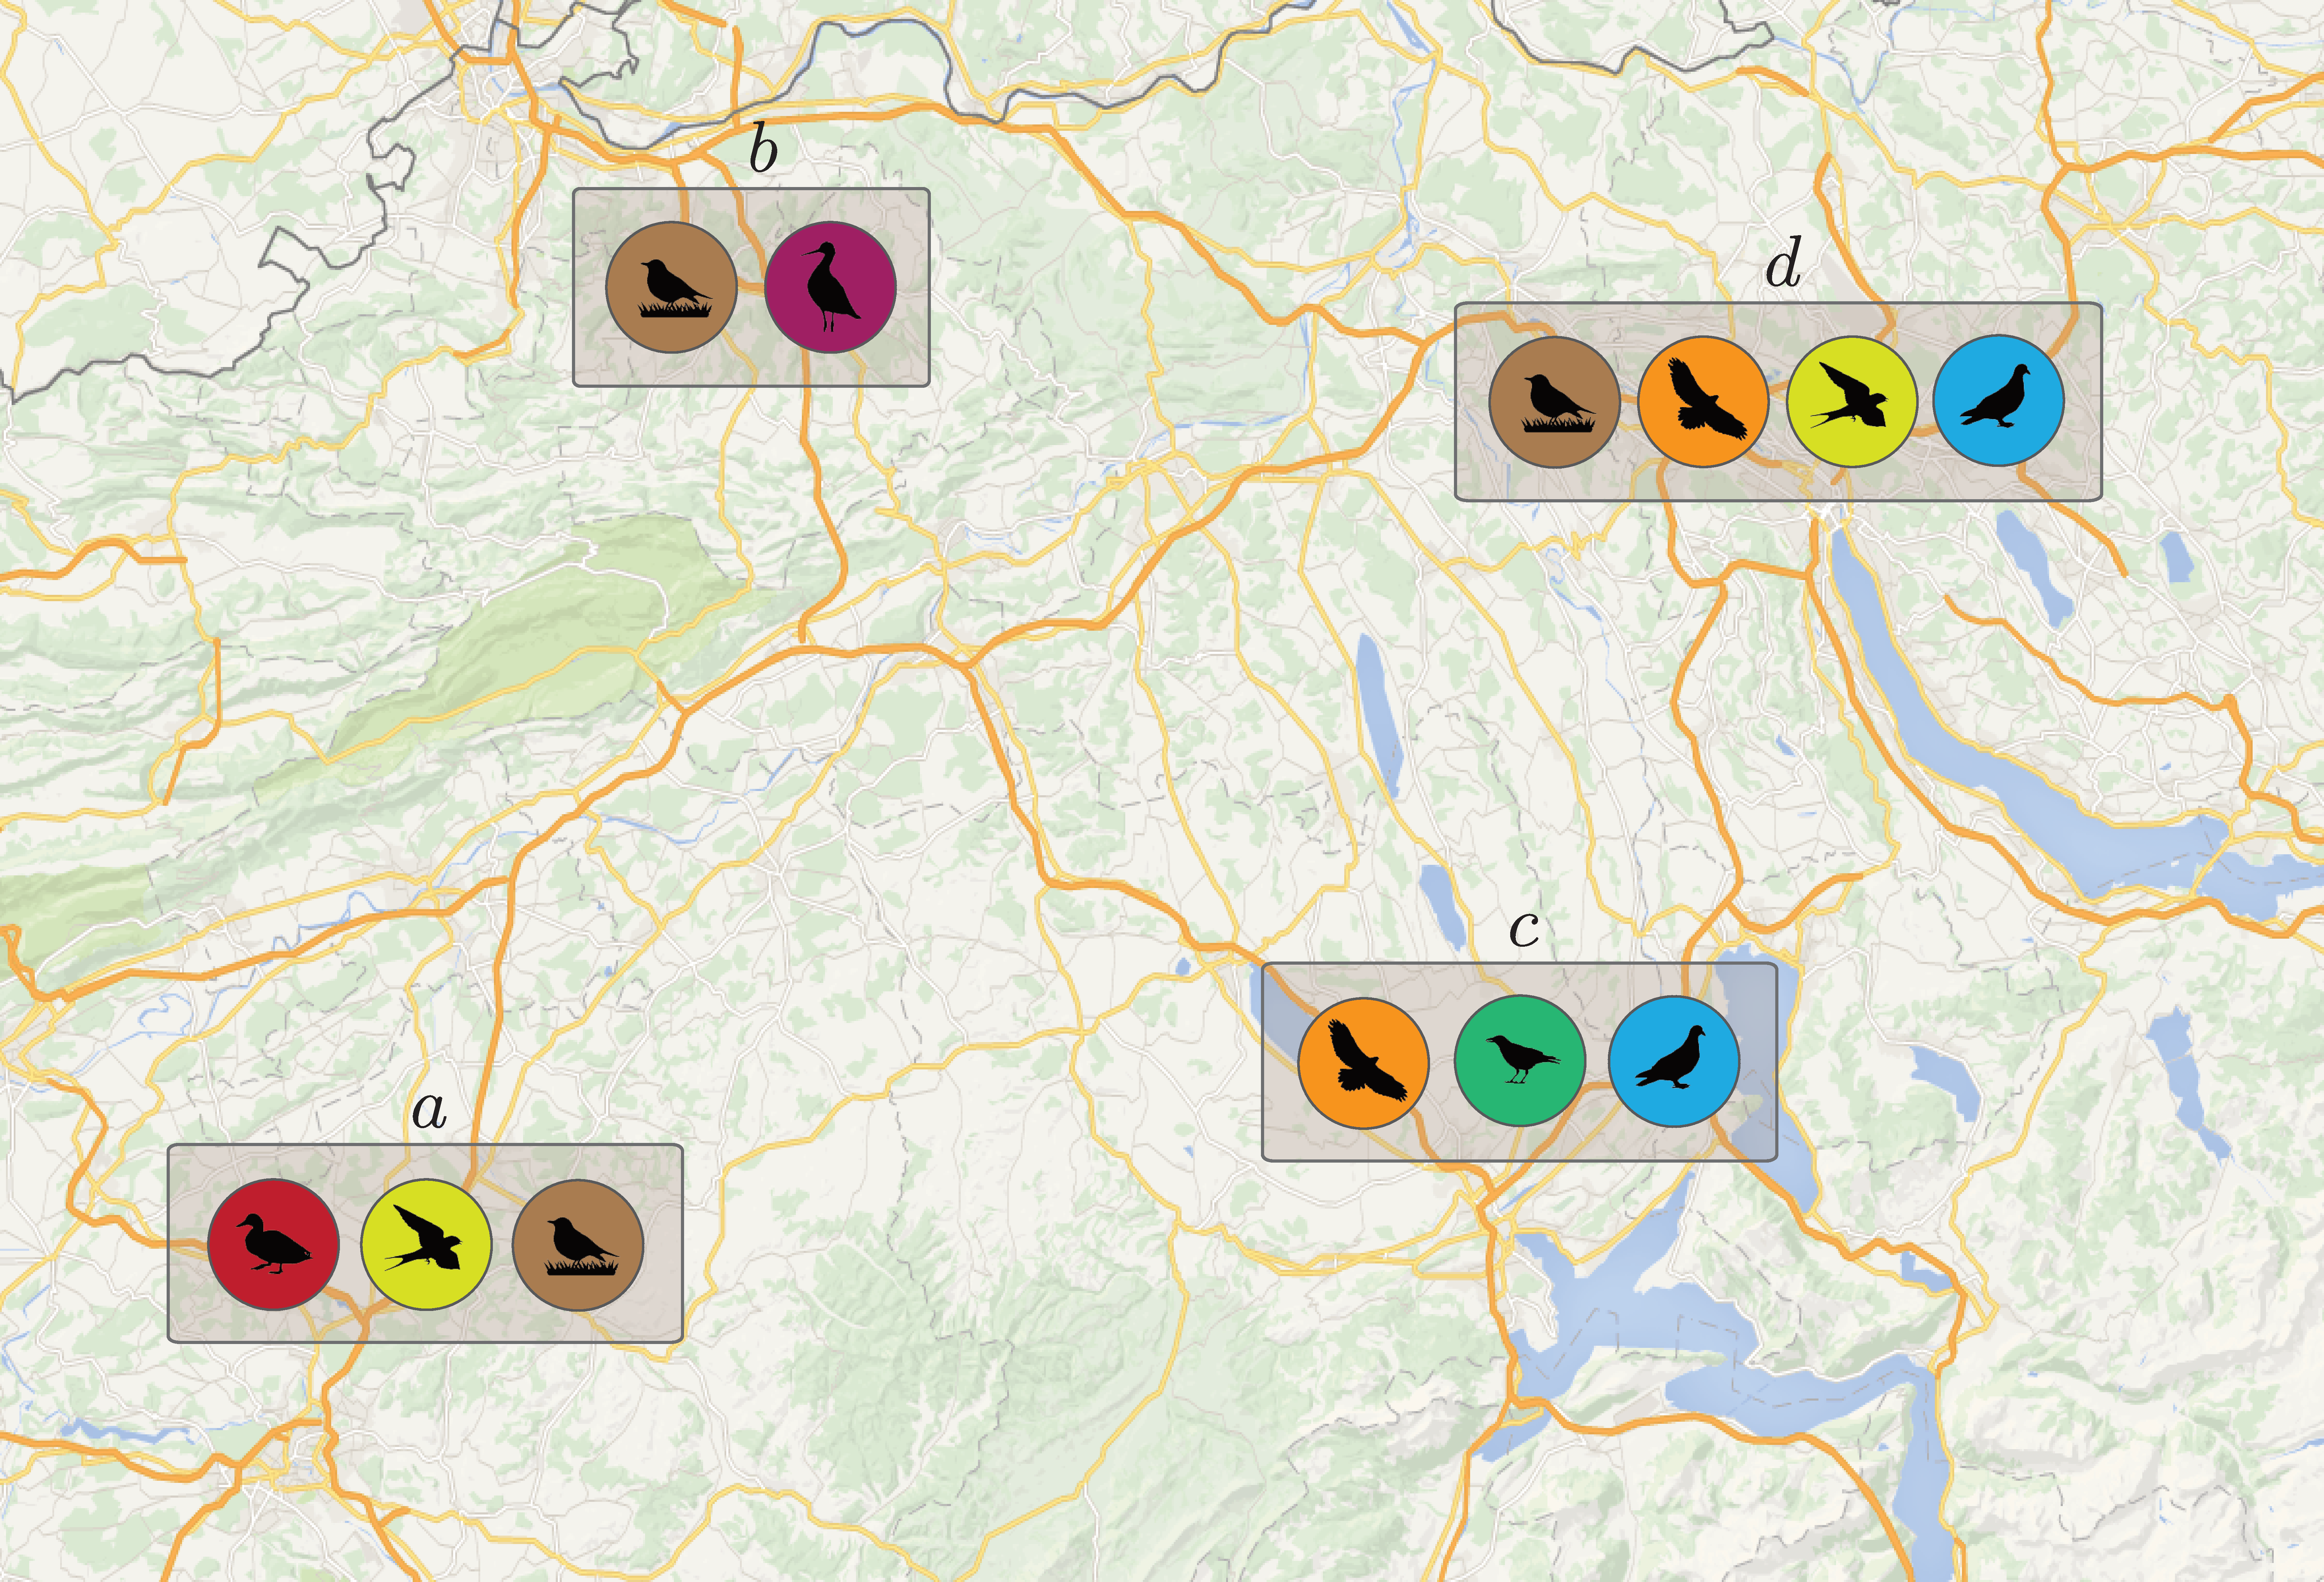
\includegraphics[width=4.75in]{figures/intro_2.pdf}
\end{frame}

\begin{frame}{Objective}
\begin{columns}[c]
\column{0.6\textwidth}
\begin{itemize}
\item Ground set $V = \{a, b, c, d\}$
\vspace{2em}
\item Objective function $f : 2^V \to \mathbb{R}_{\geq 0}$
\vspace{2em}
\item $f(\{c\}) = 3$
\vspace{2em}
\item $f(\{a, c\}) = 4$
\end{itemize}
\column{0.4\textwidth}
\centering
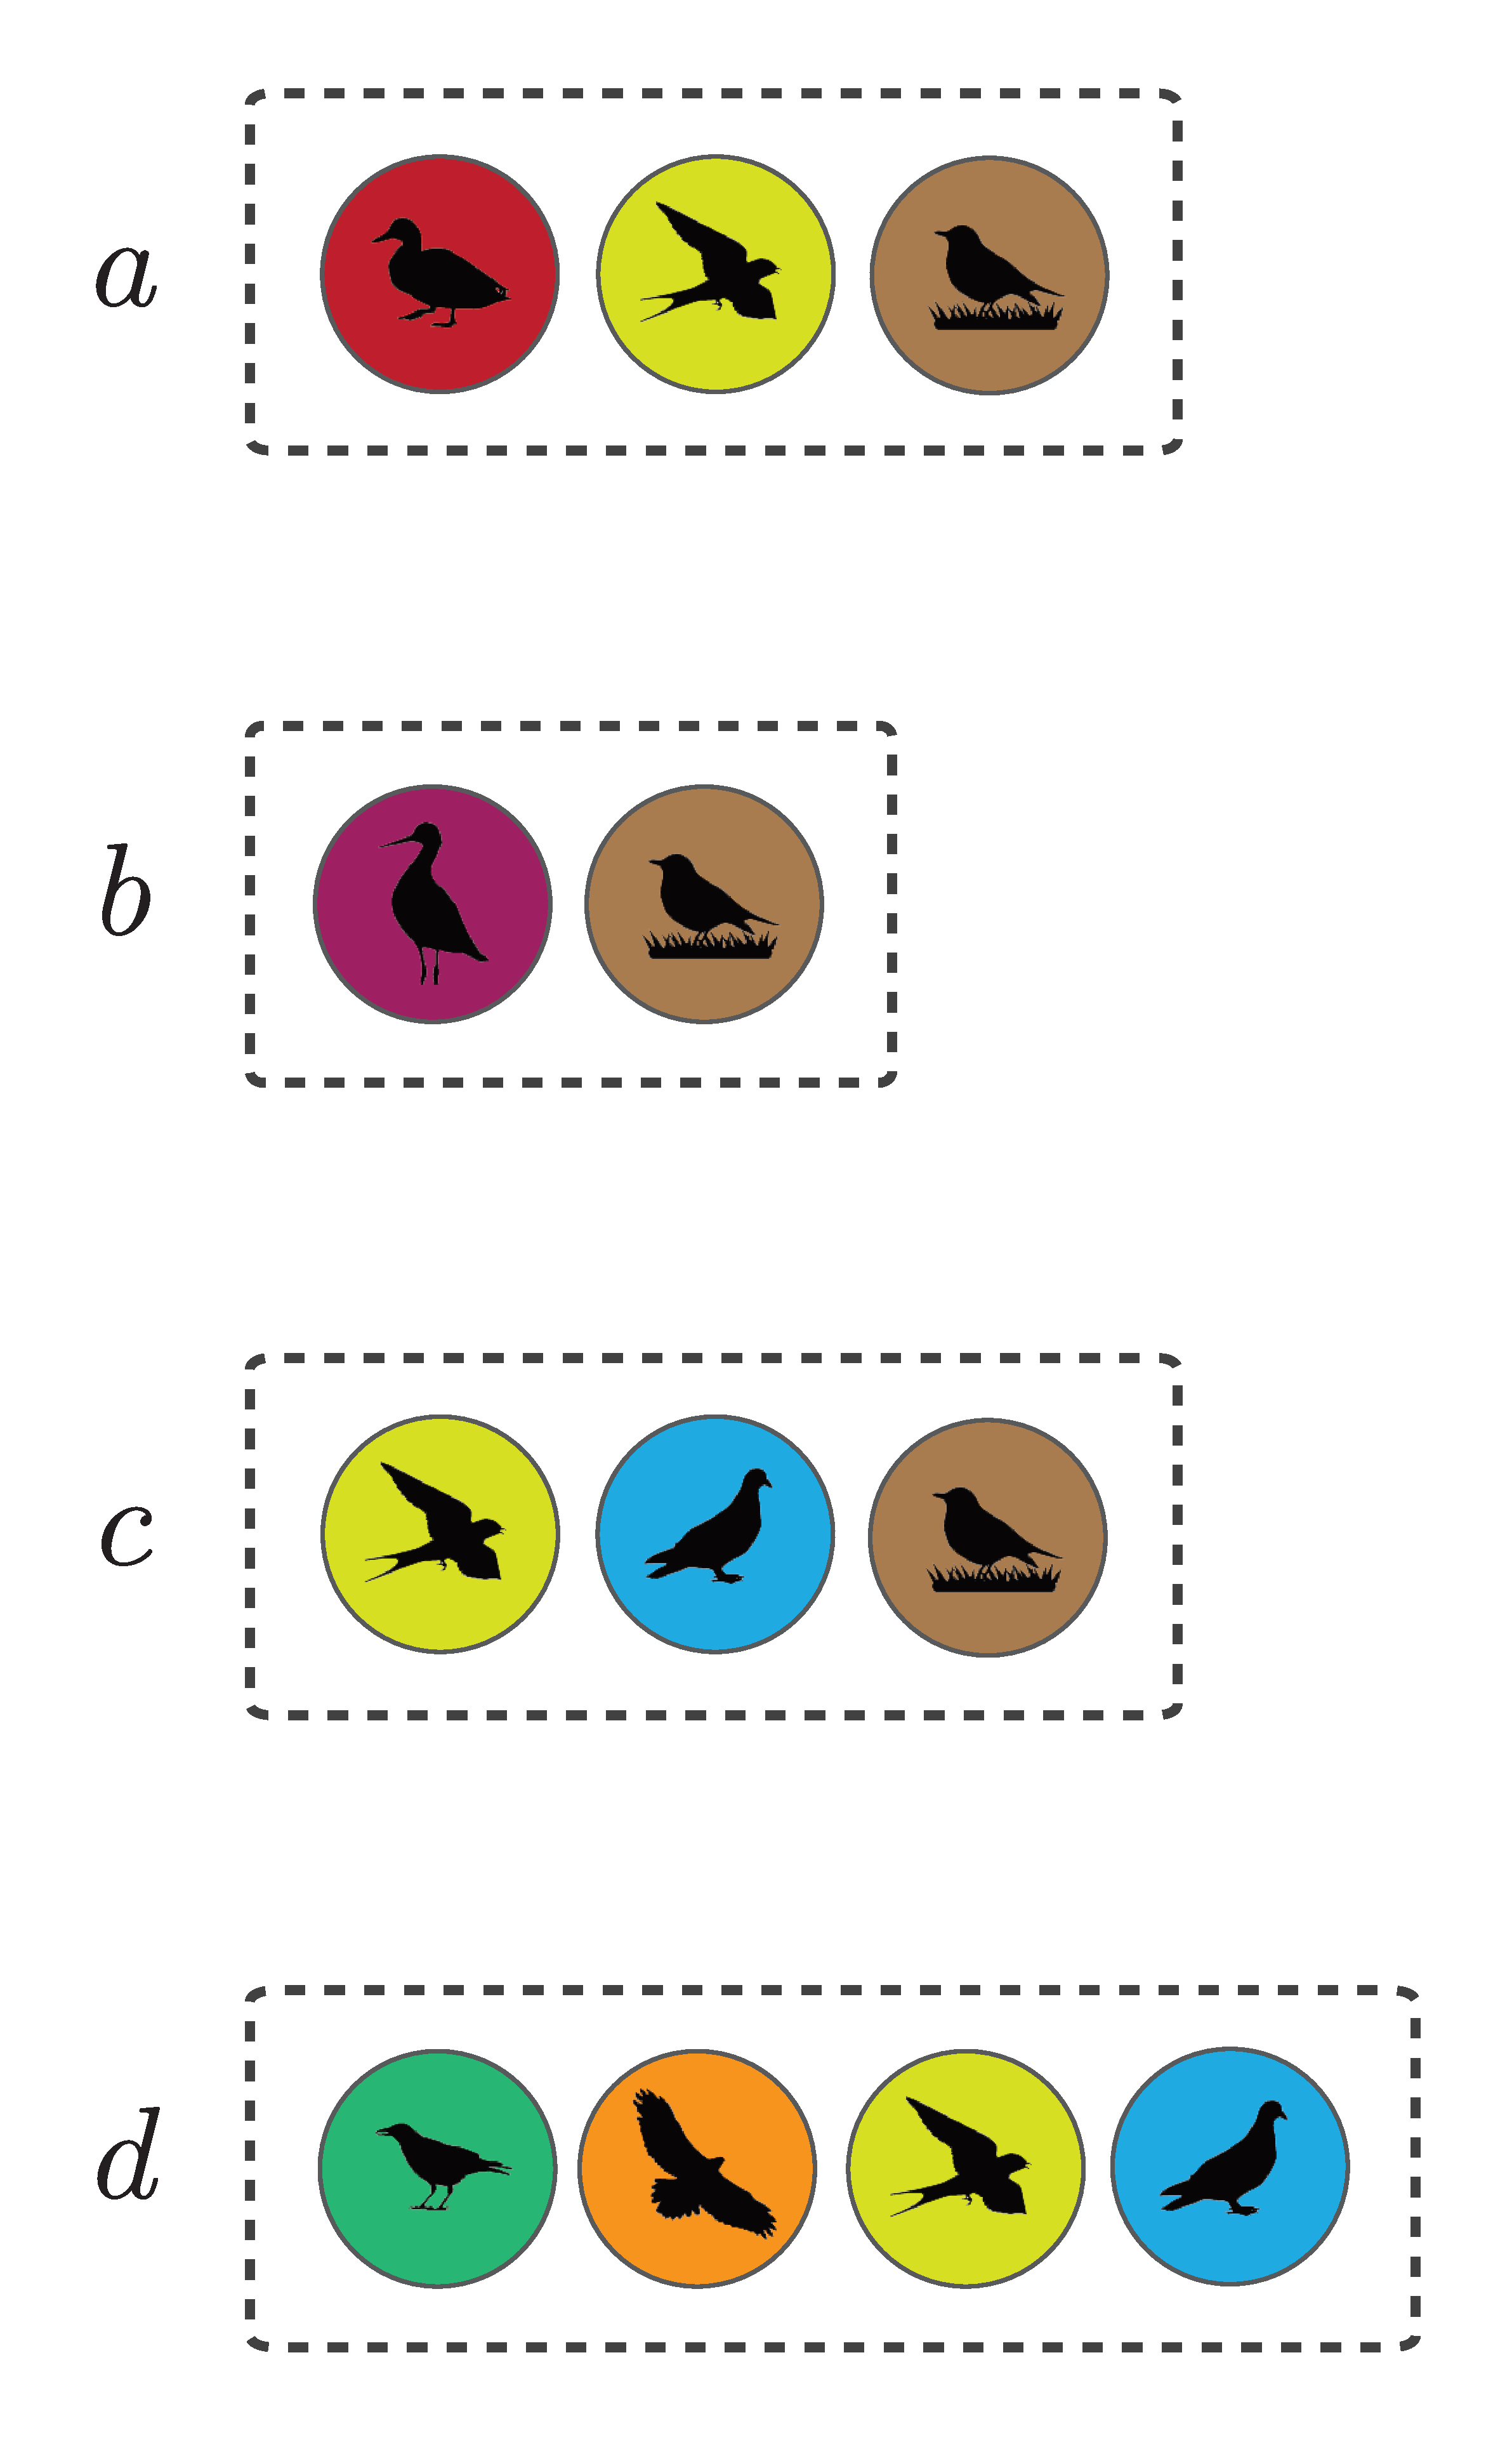
\includegraphics[width=2in]{figures/sets.pdf}
\end{columns}
\end{frame}

\begin{frame}{Objective}
\begin{columns}[c]
\column{0.6\textwidth}
\begin{itemize}
\item $f$ is monotone
\vspace{2em}
\item $f$ is submodular
\vspace{2em}
\item Benefit of visiting $c$, given that\ldots
\begin{itemize}
\vspace{1em}
\item \ldots it is the first place we visit:
\begin{align*}
  f(\{c\}) = 3
\end{align*}
\item \ldots we have already visited $d$:
\begin{align*}
  f(\{c, d\}) - f(\{d\}) = 4 - 3 = 1
\end{align*}
\end{itemize}
\end{itemize}
\column{0.4\textwidth}
\centering
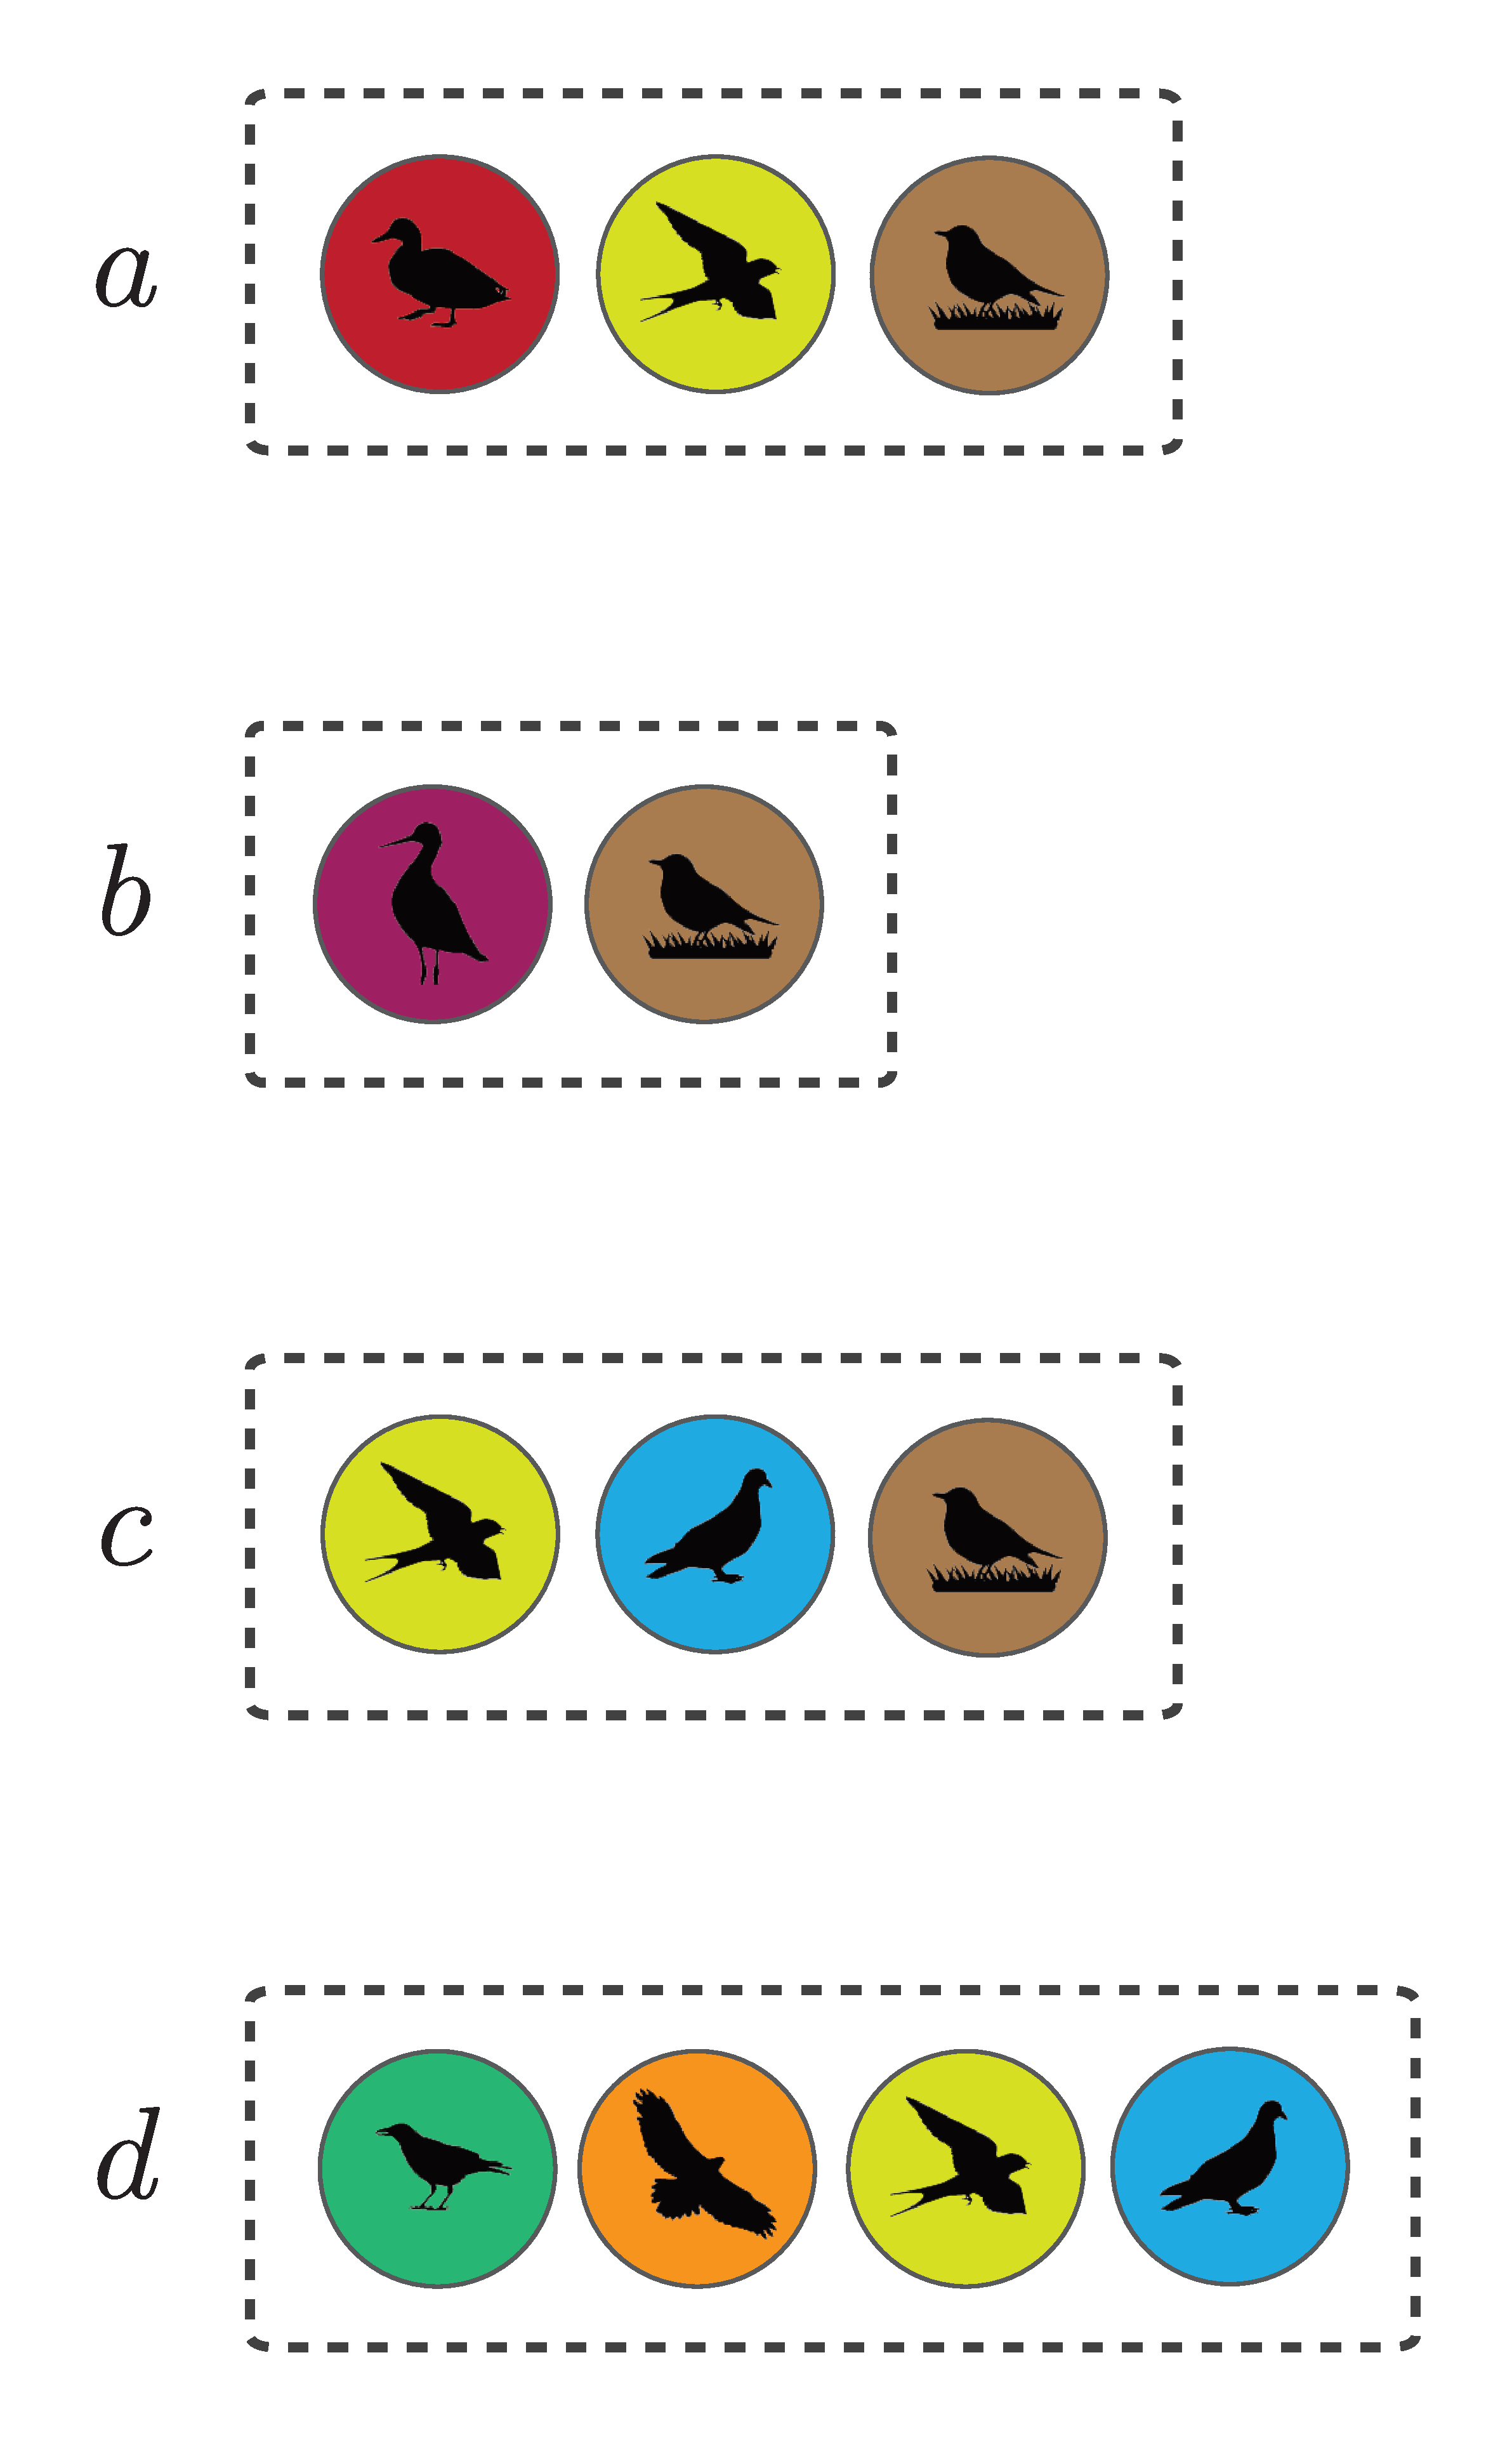
\includegraphics[width=2in]{figures/sets.pdf}
\end{columns}
\end{frame}

\renewcommand{\tabularxcolumn}[1]{>{\small}m{#1}}
\begin{frame}{Monotone submodular maximization}
\begin{itemize}
\item Unconstrained problem:\\
\begin{tabularx}{3in}{XcX}
{\begin{align*}\textrm{maximize}\ \ \ f(S)\end{align*}} & $\longrightarrow$ & {\color{green!50!darkgray}Trivial} $\ \ \textrm{OPT} = f(V)$
\end{tabularx}
\vspace{2em}
\item Cardinality-constrained problem:\\
\begin{tabularx}{3in}{XcX}
{\begin{align*}\textrm{maximize}\ \ \ &f(S)\\ \textrm{subject to}\ \ \ &|S| \leq k\end{align*}} & $\longrightarrow$ & \color{red!80!darkgray} NP-hard
\end{tabularx}
\end{itemize}
\end{frame}

\begin{frame}{Greedy}
\begin{columns}[c]
\column{0.6\textwidth}
\begin{itemize}
\item<1-> $k = 3$
\vspace{1em}
\item<2-> $S_0 = \varnothing\ \ \longrightarrow\ \ f(S_0) = 0$
\vspace{1em}
\item<3-> $S_1 = \{d\}\ \ \longrightarrow\ \ f(S_1) = 4$
\vspace{1em}
\item<4-> $S_2 = \{d, a\}\ \ \longrightarrow\ \ f(S_2) = 5$
\vspace{1em}
\item<5-> $S_3 = \{d, a, b\}\ \ \longrightarrow\ \ f(S_3) = 6$
\vspace{1em}
\item<6-> $\textrm{OPT} = f(\{a, b, c\}) = 7$
\end{itemize}
\column{0.4\textwidth}
\centering
\only<1-2>{
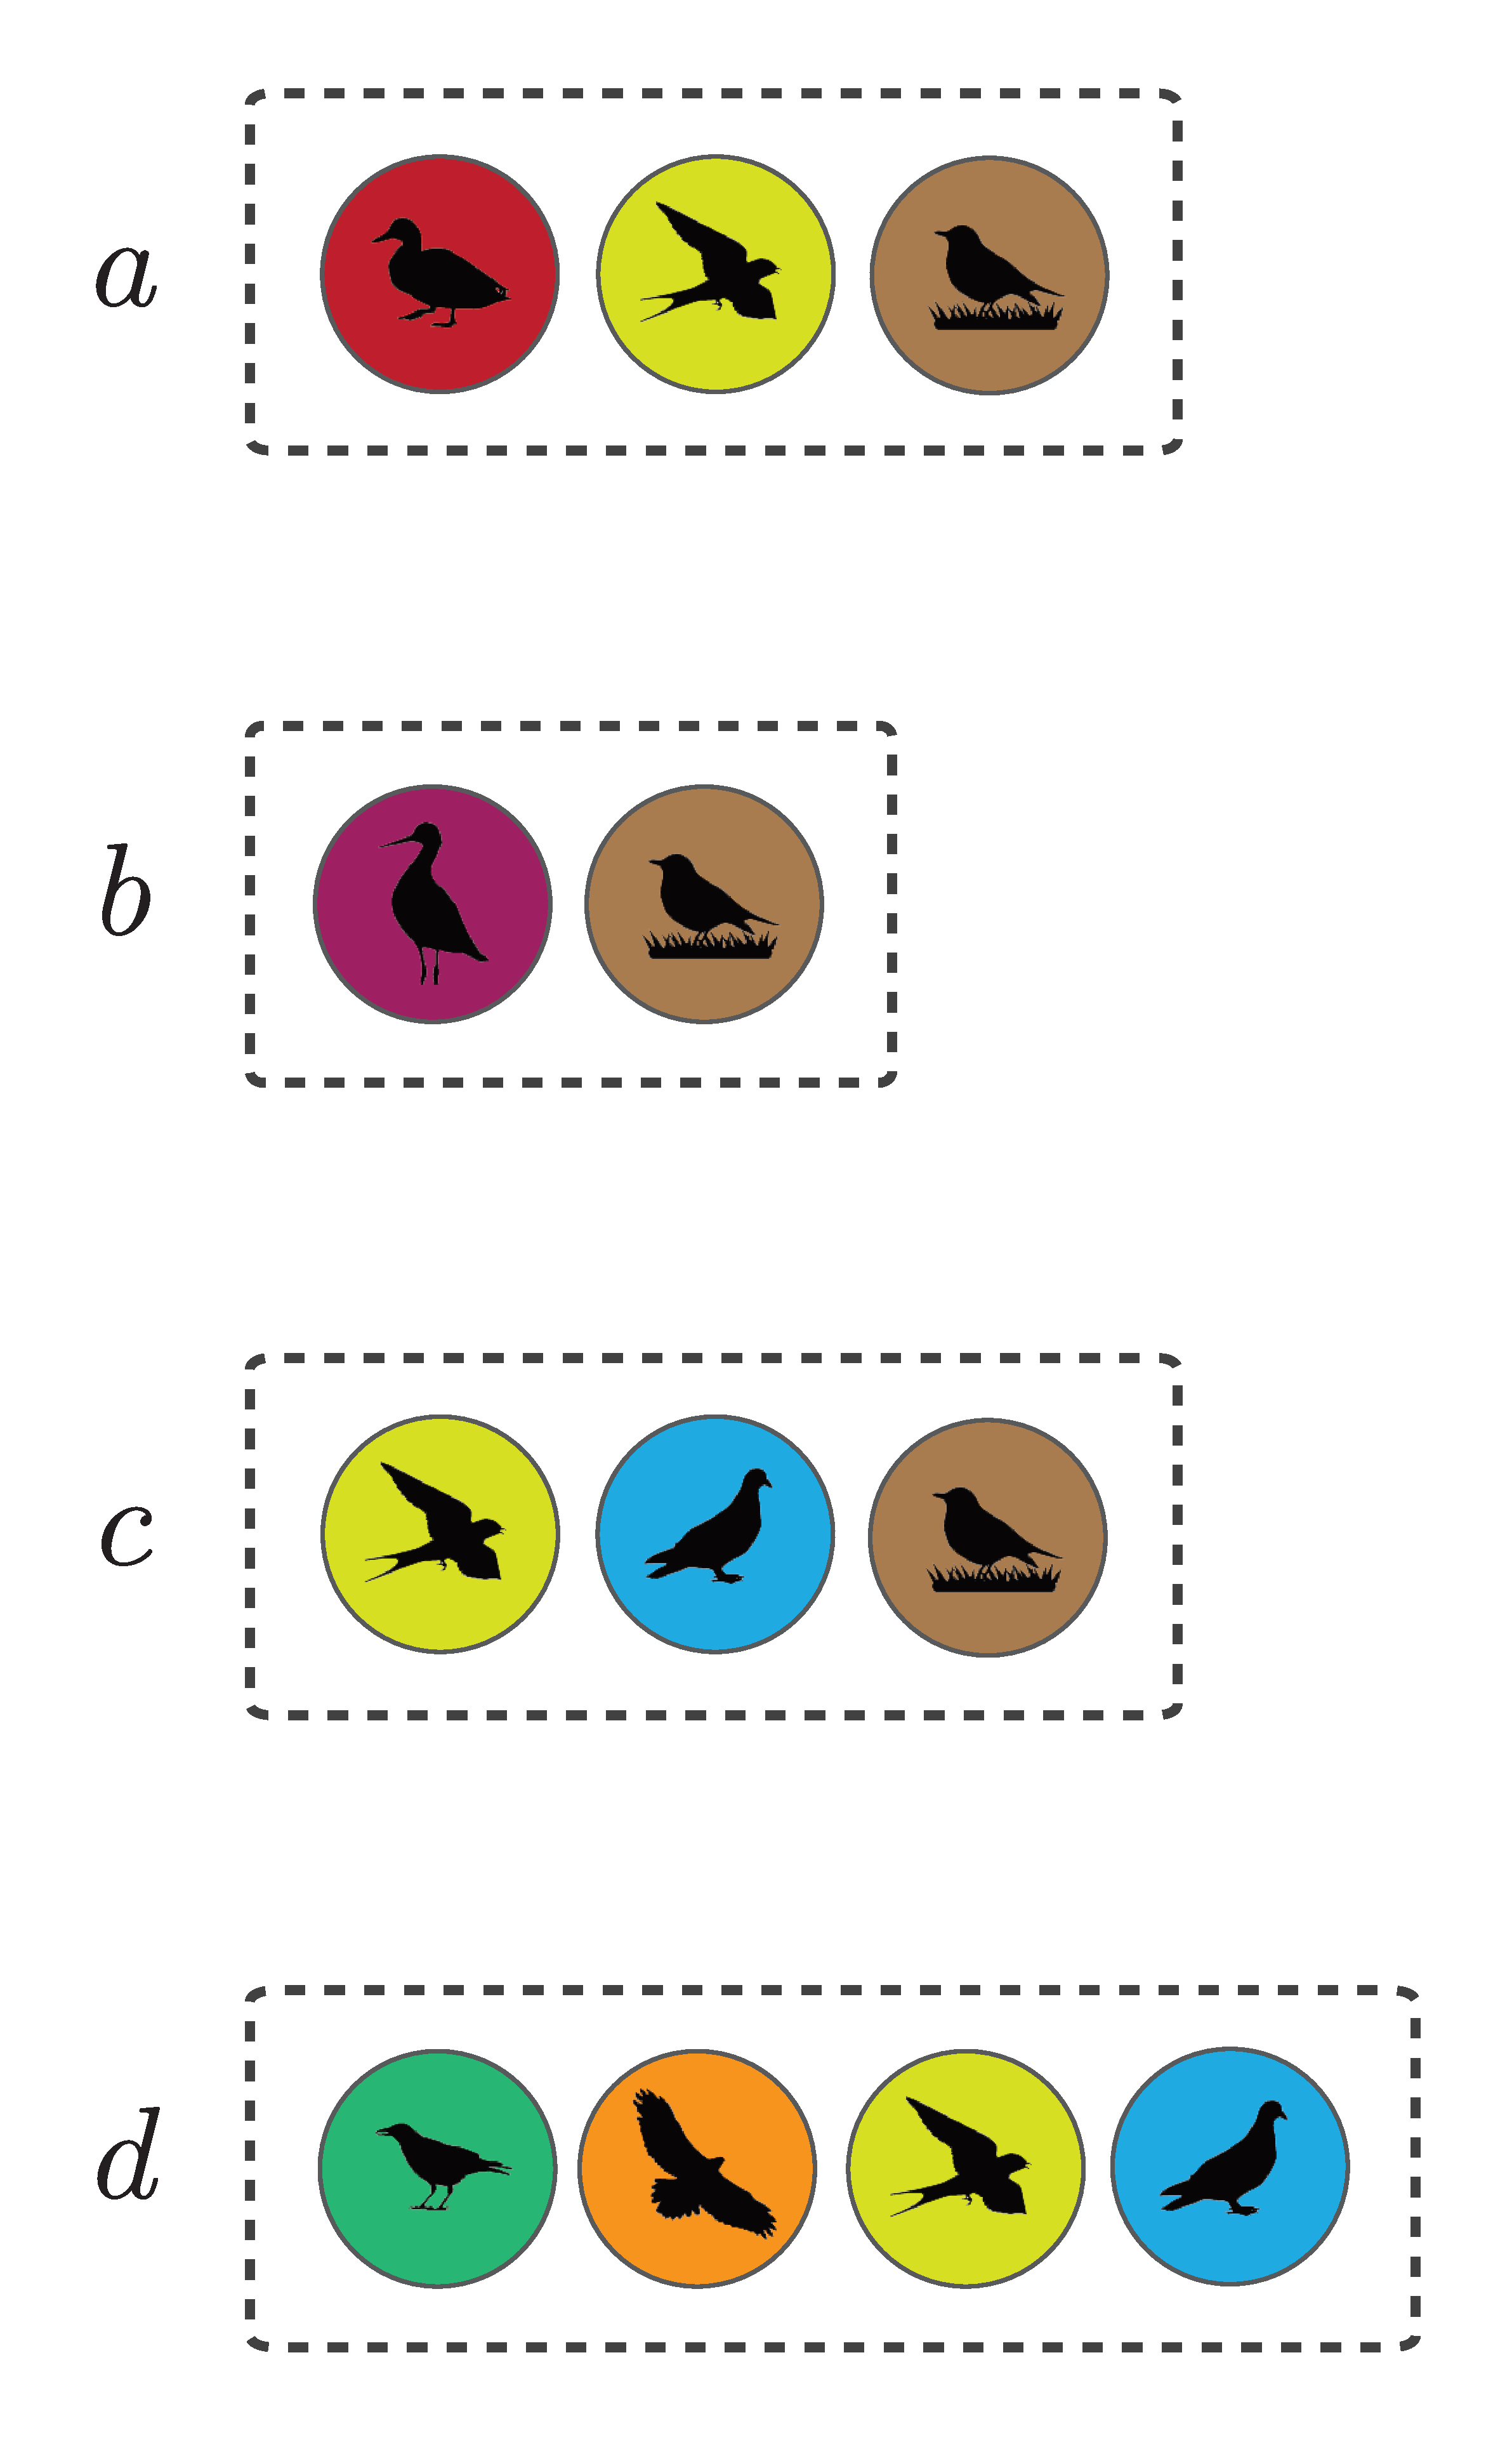
\includegraphics[width=2in]{figures/sets.pdf}
}
\only<3>{
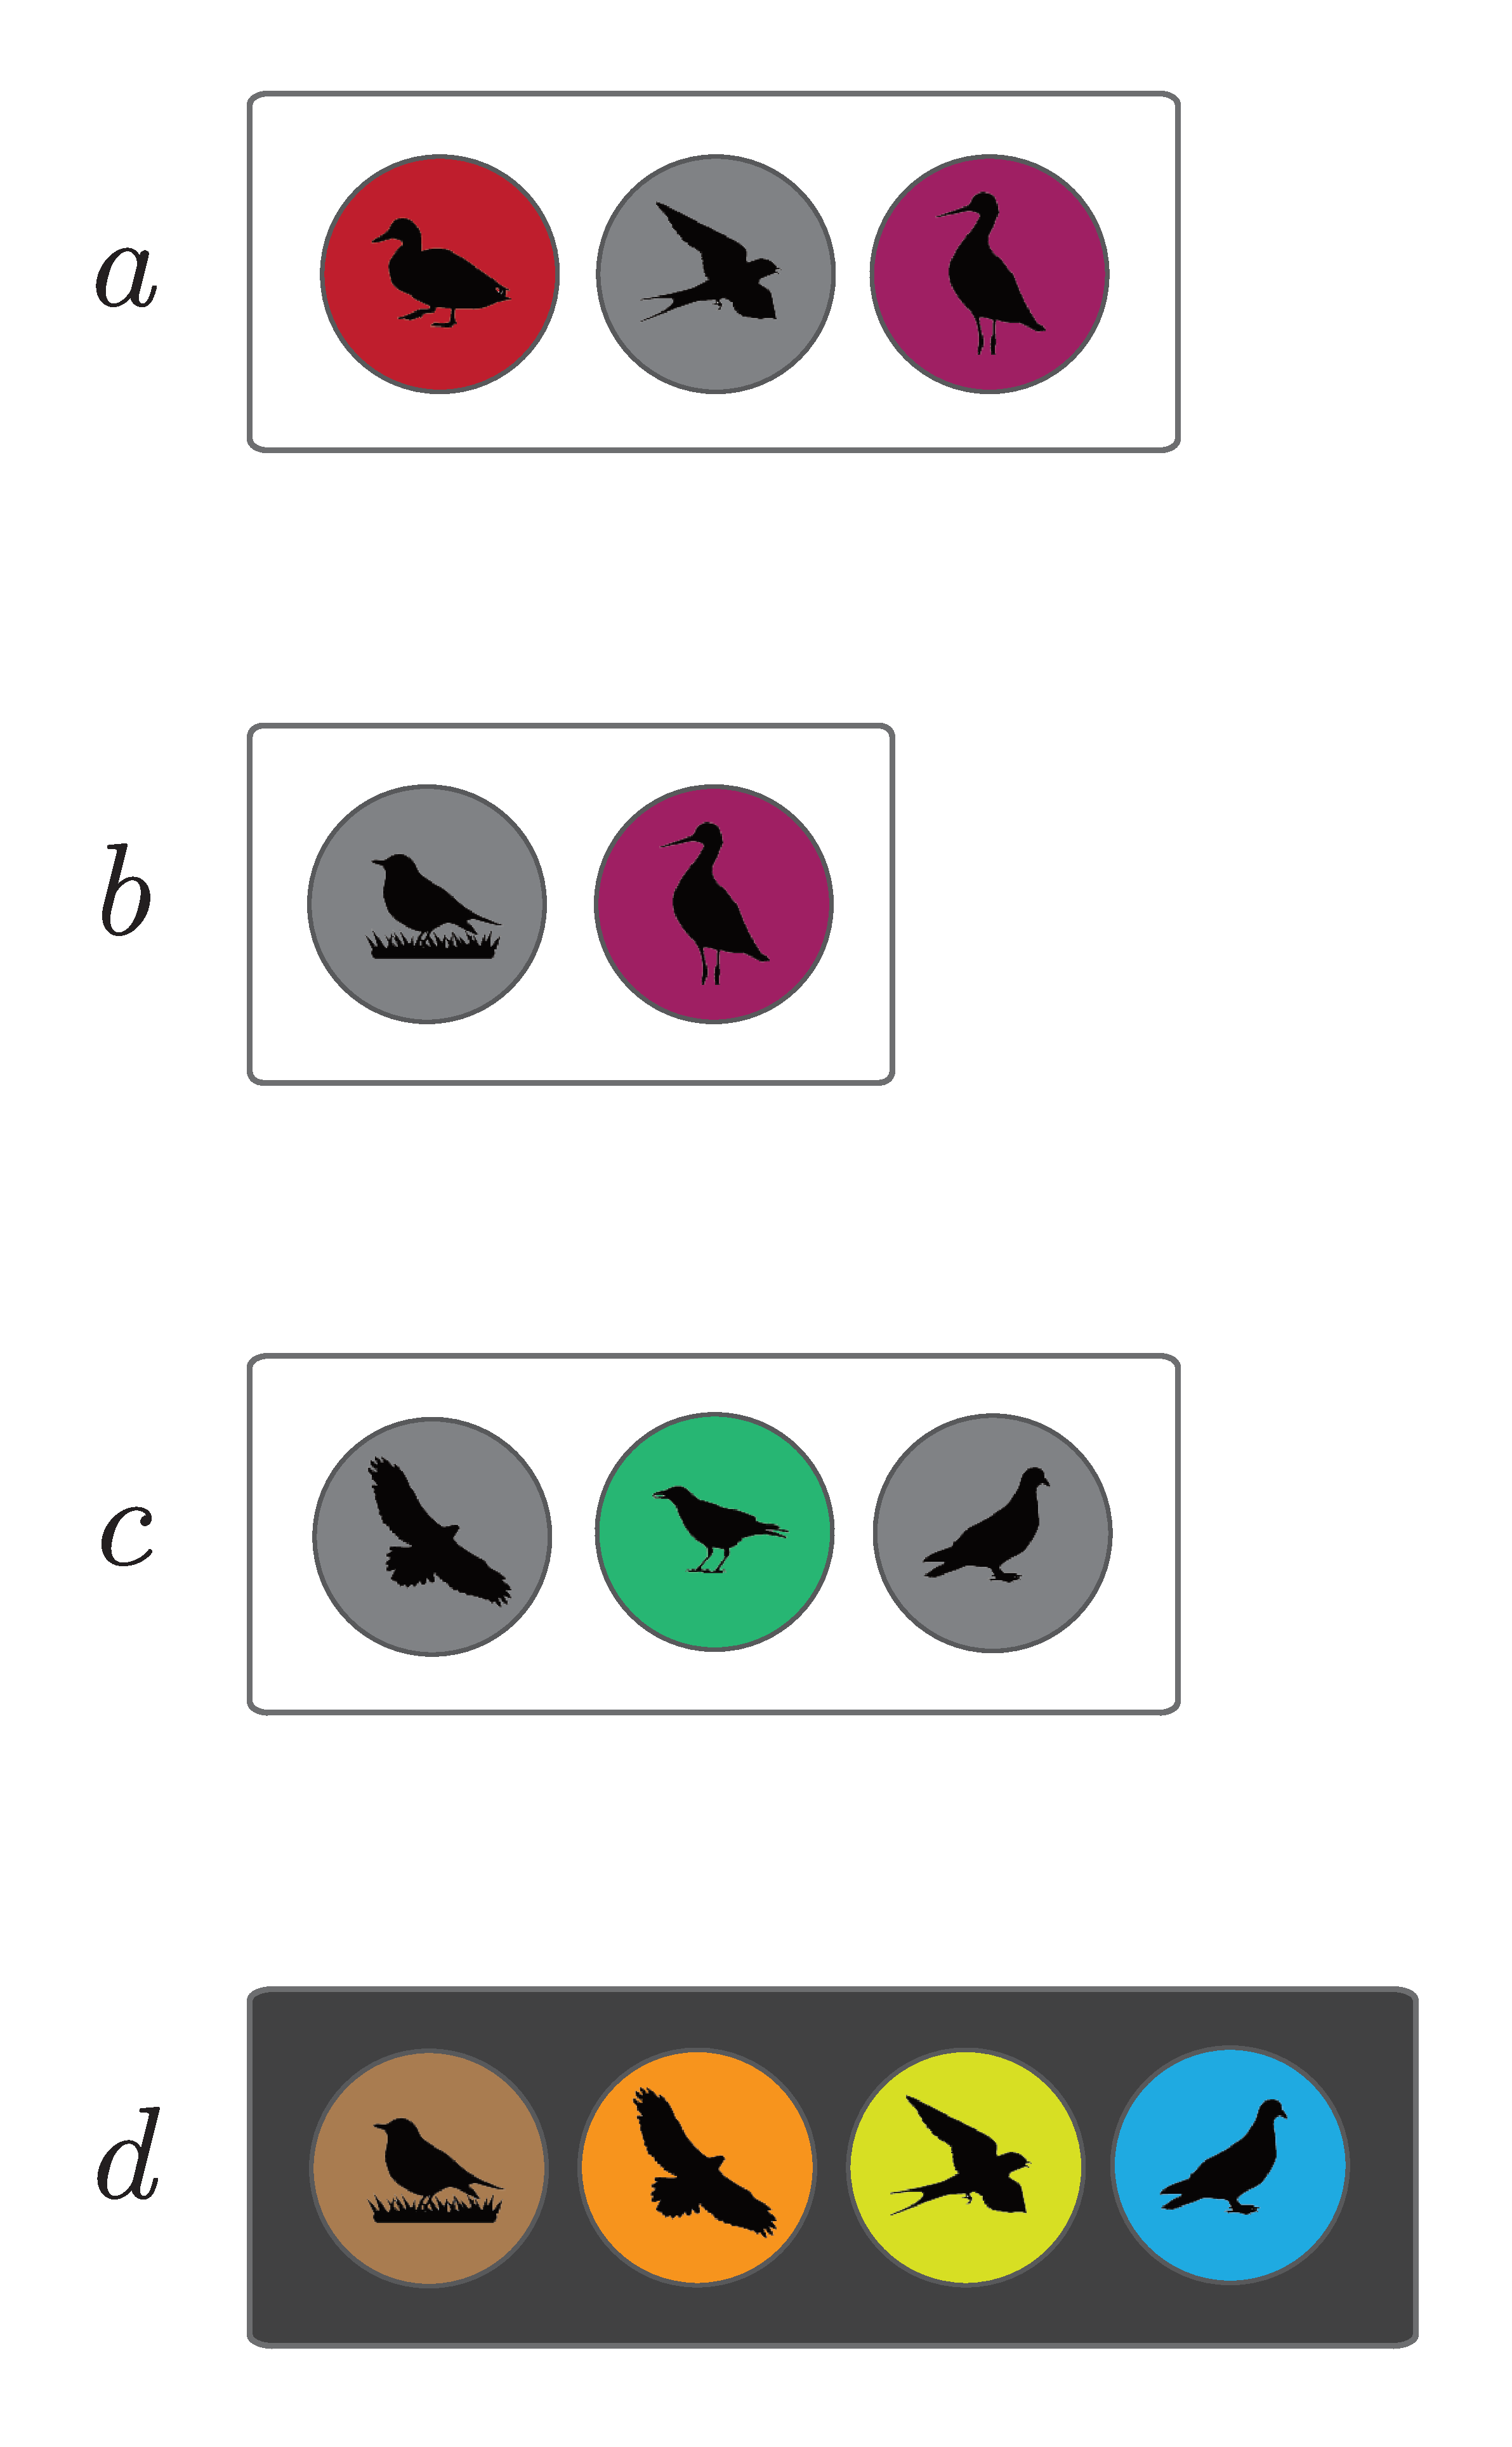
\includegraphics[width=2in]{figures/sets_greedy_1.pdf}
}
\only<4>{
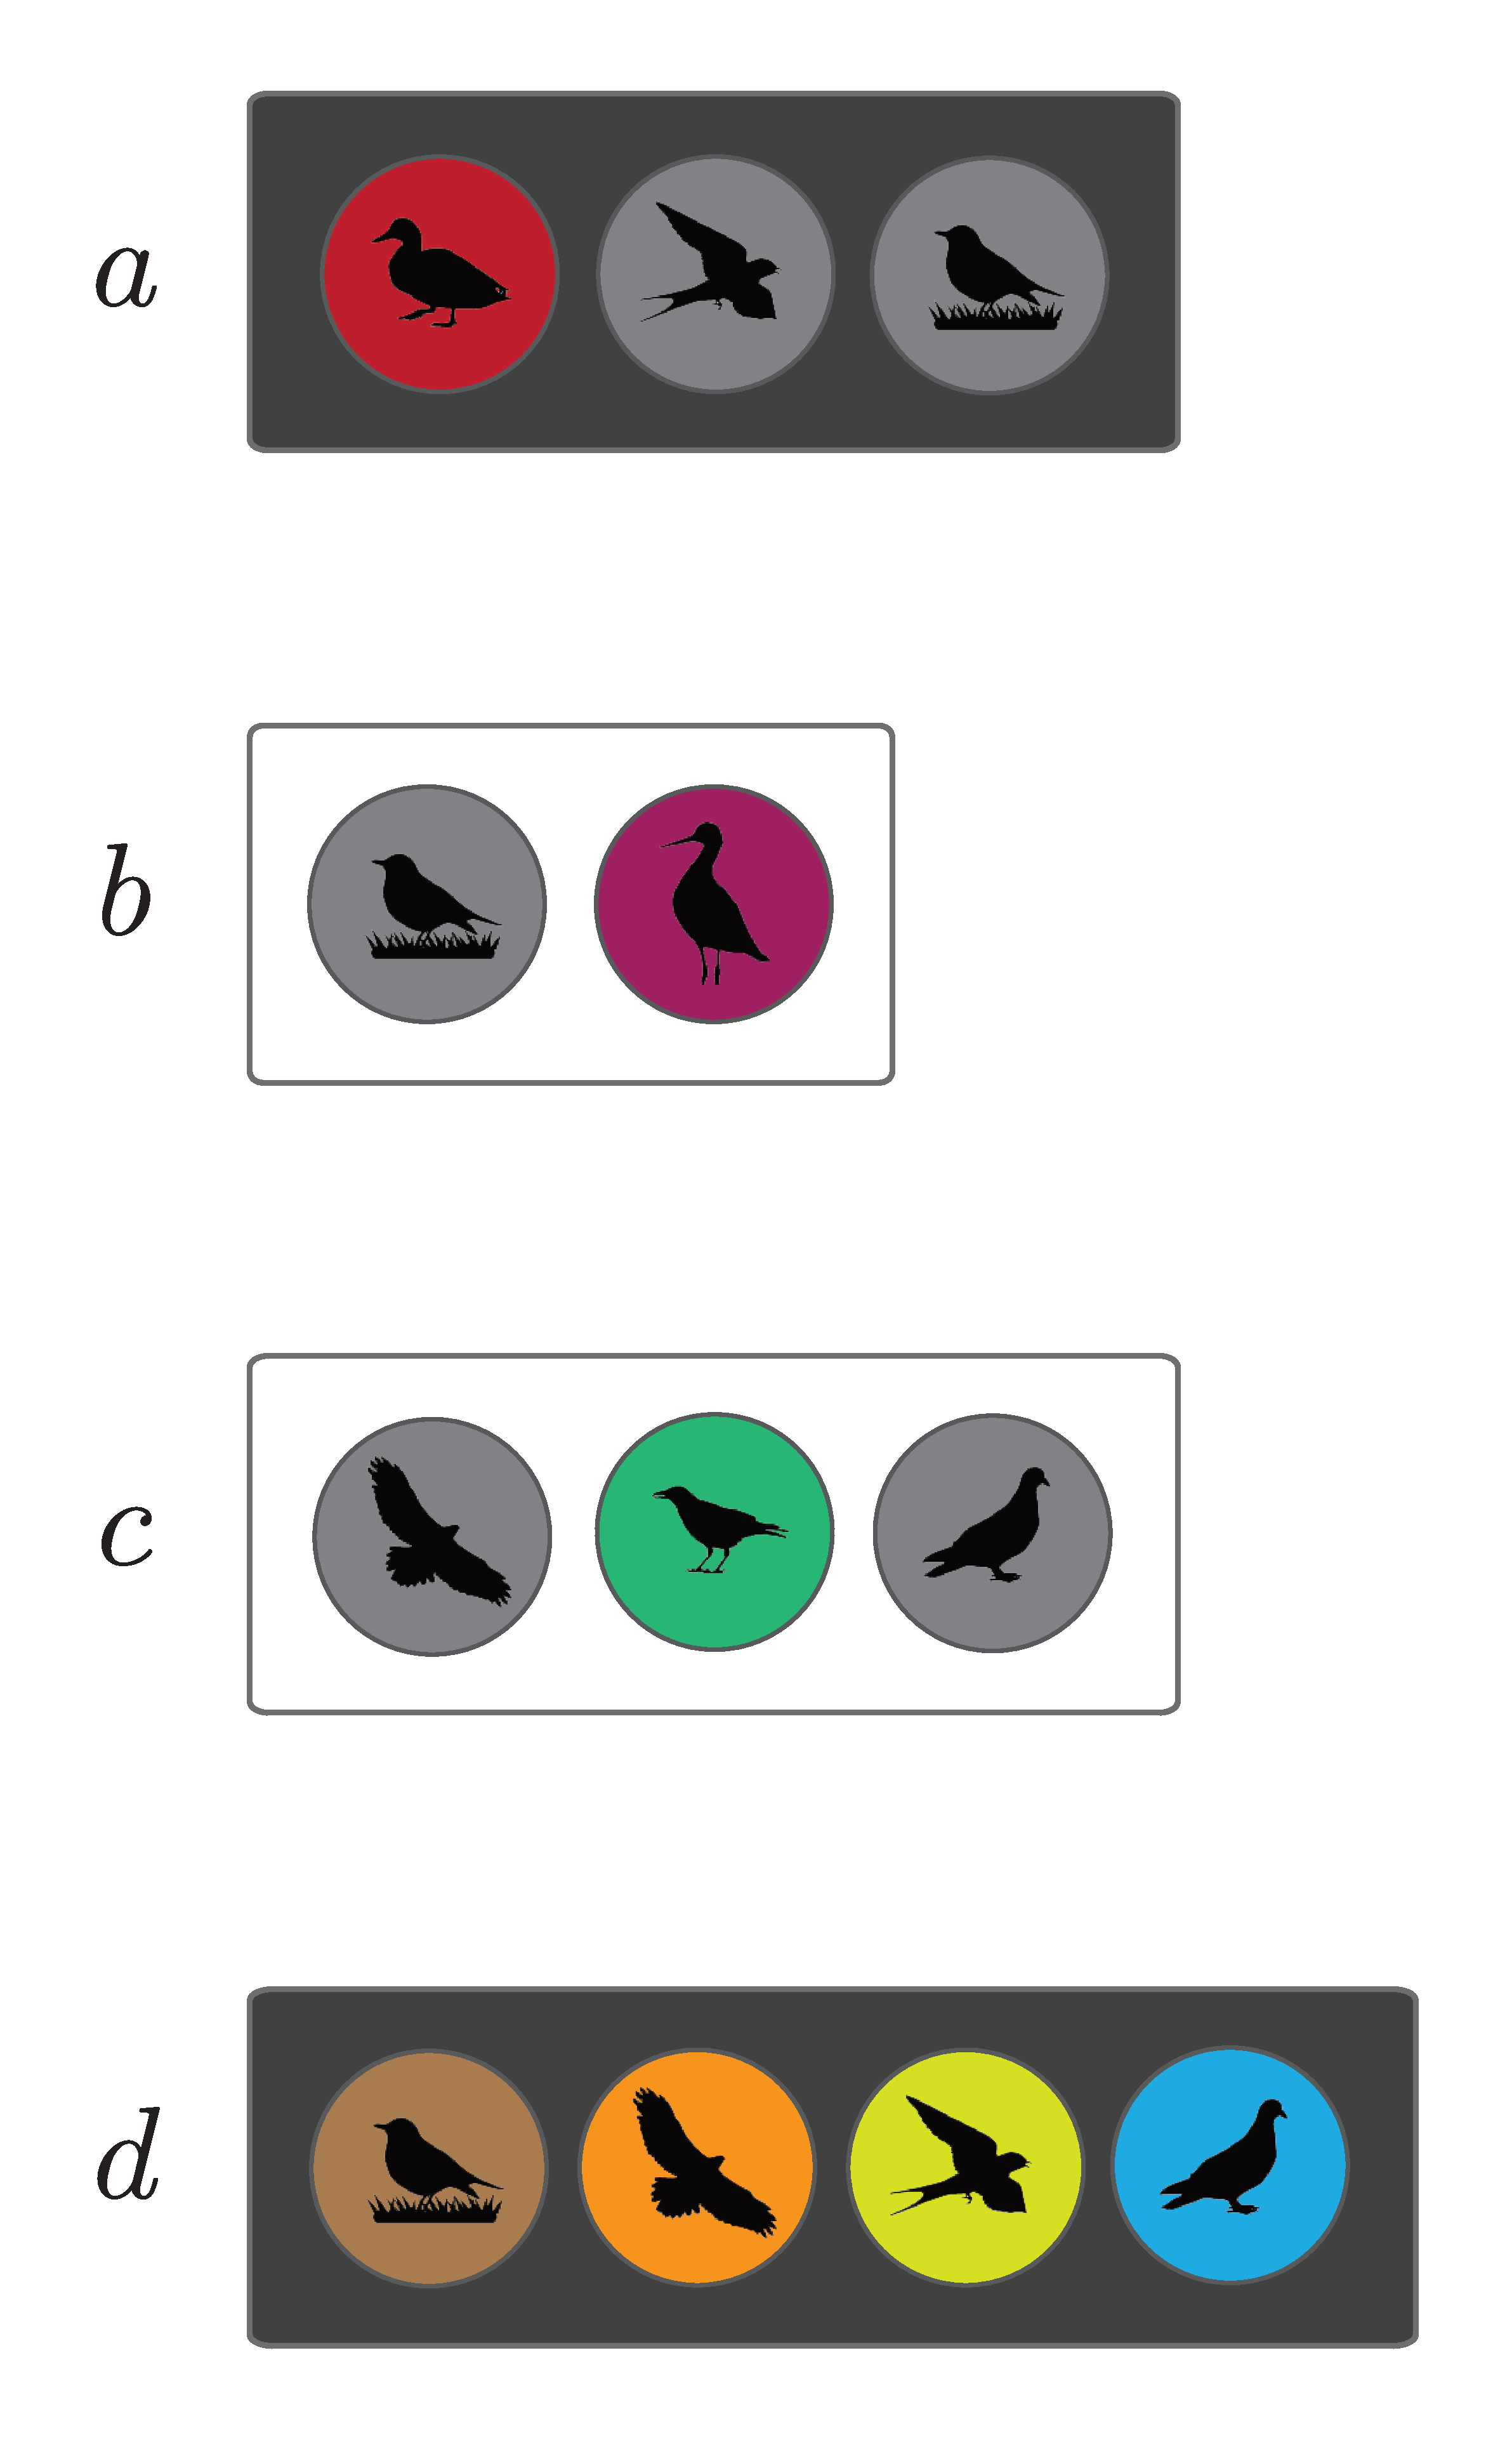
\includegraphics[width=2in]{figures/sets_greedy_2.pdf}
}
\only<5>{
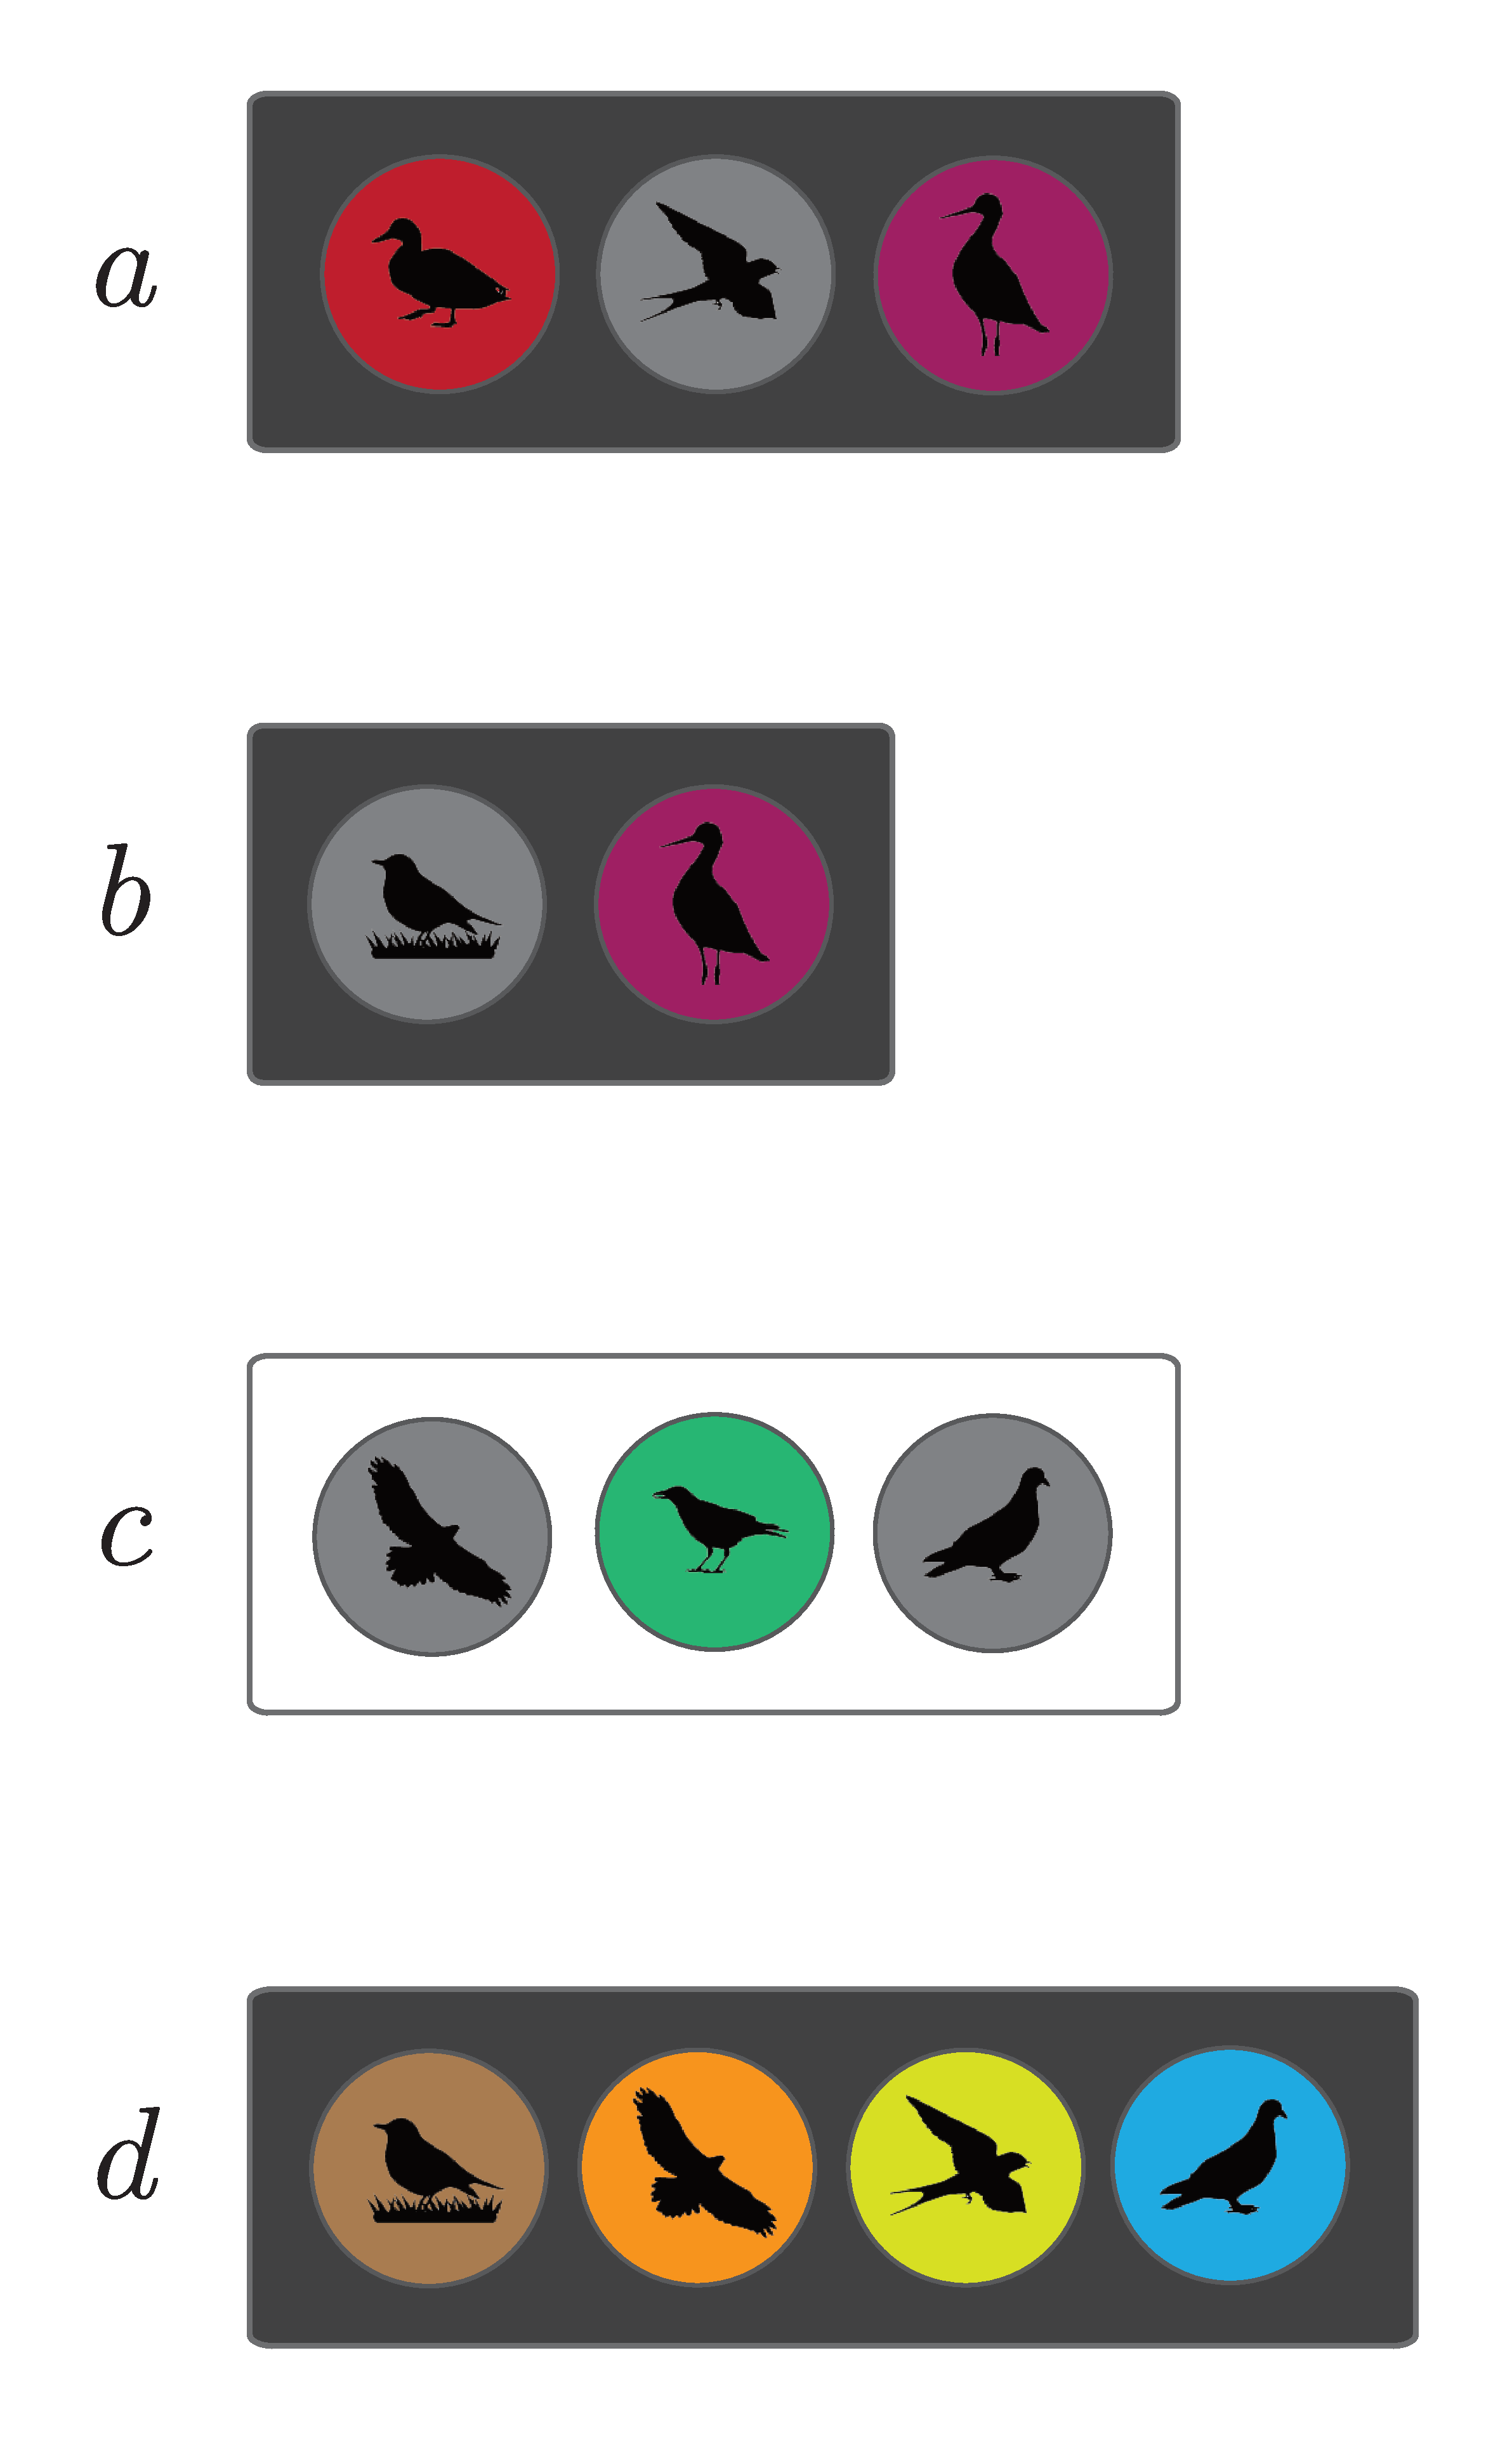
\includegraphics[width=2in]{figures/sets_greedy_3.pdf}
}
\only<6>{
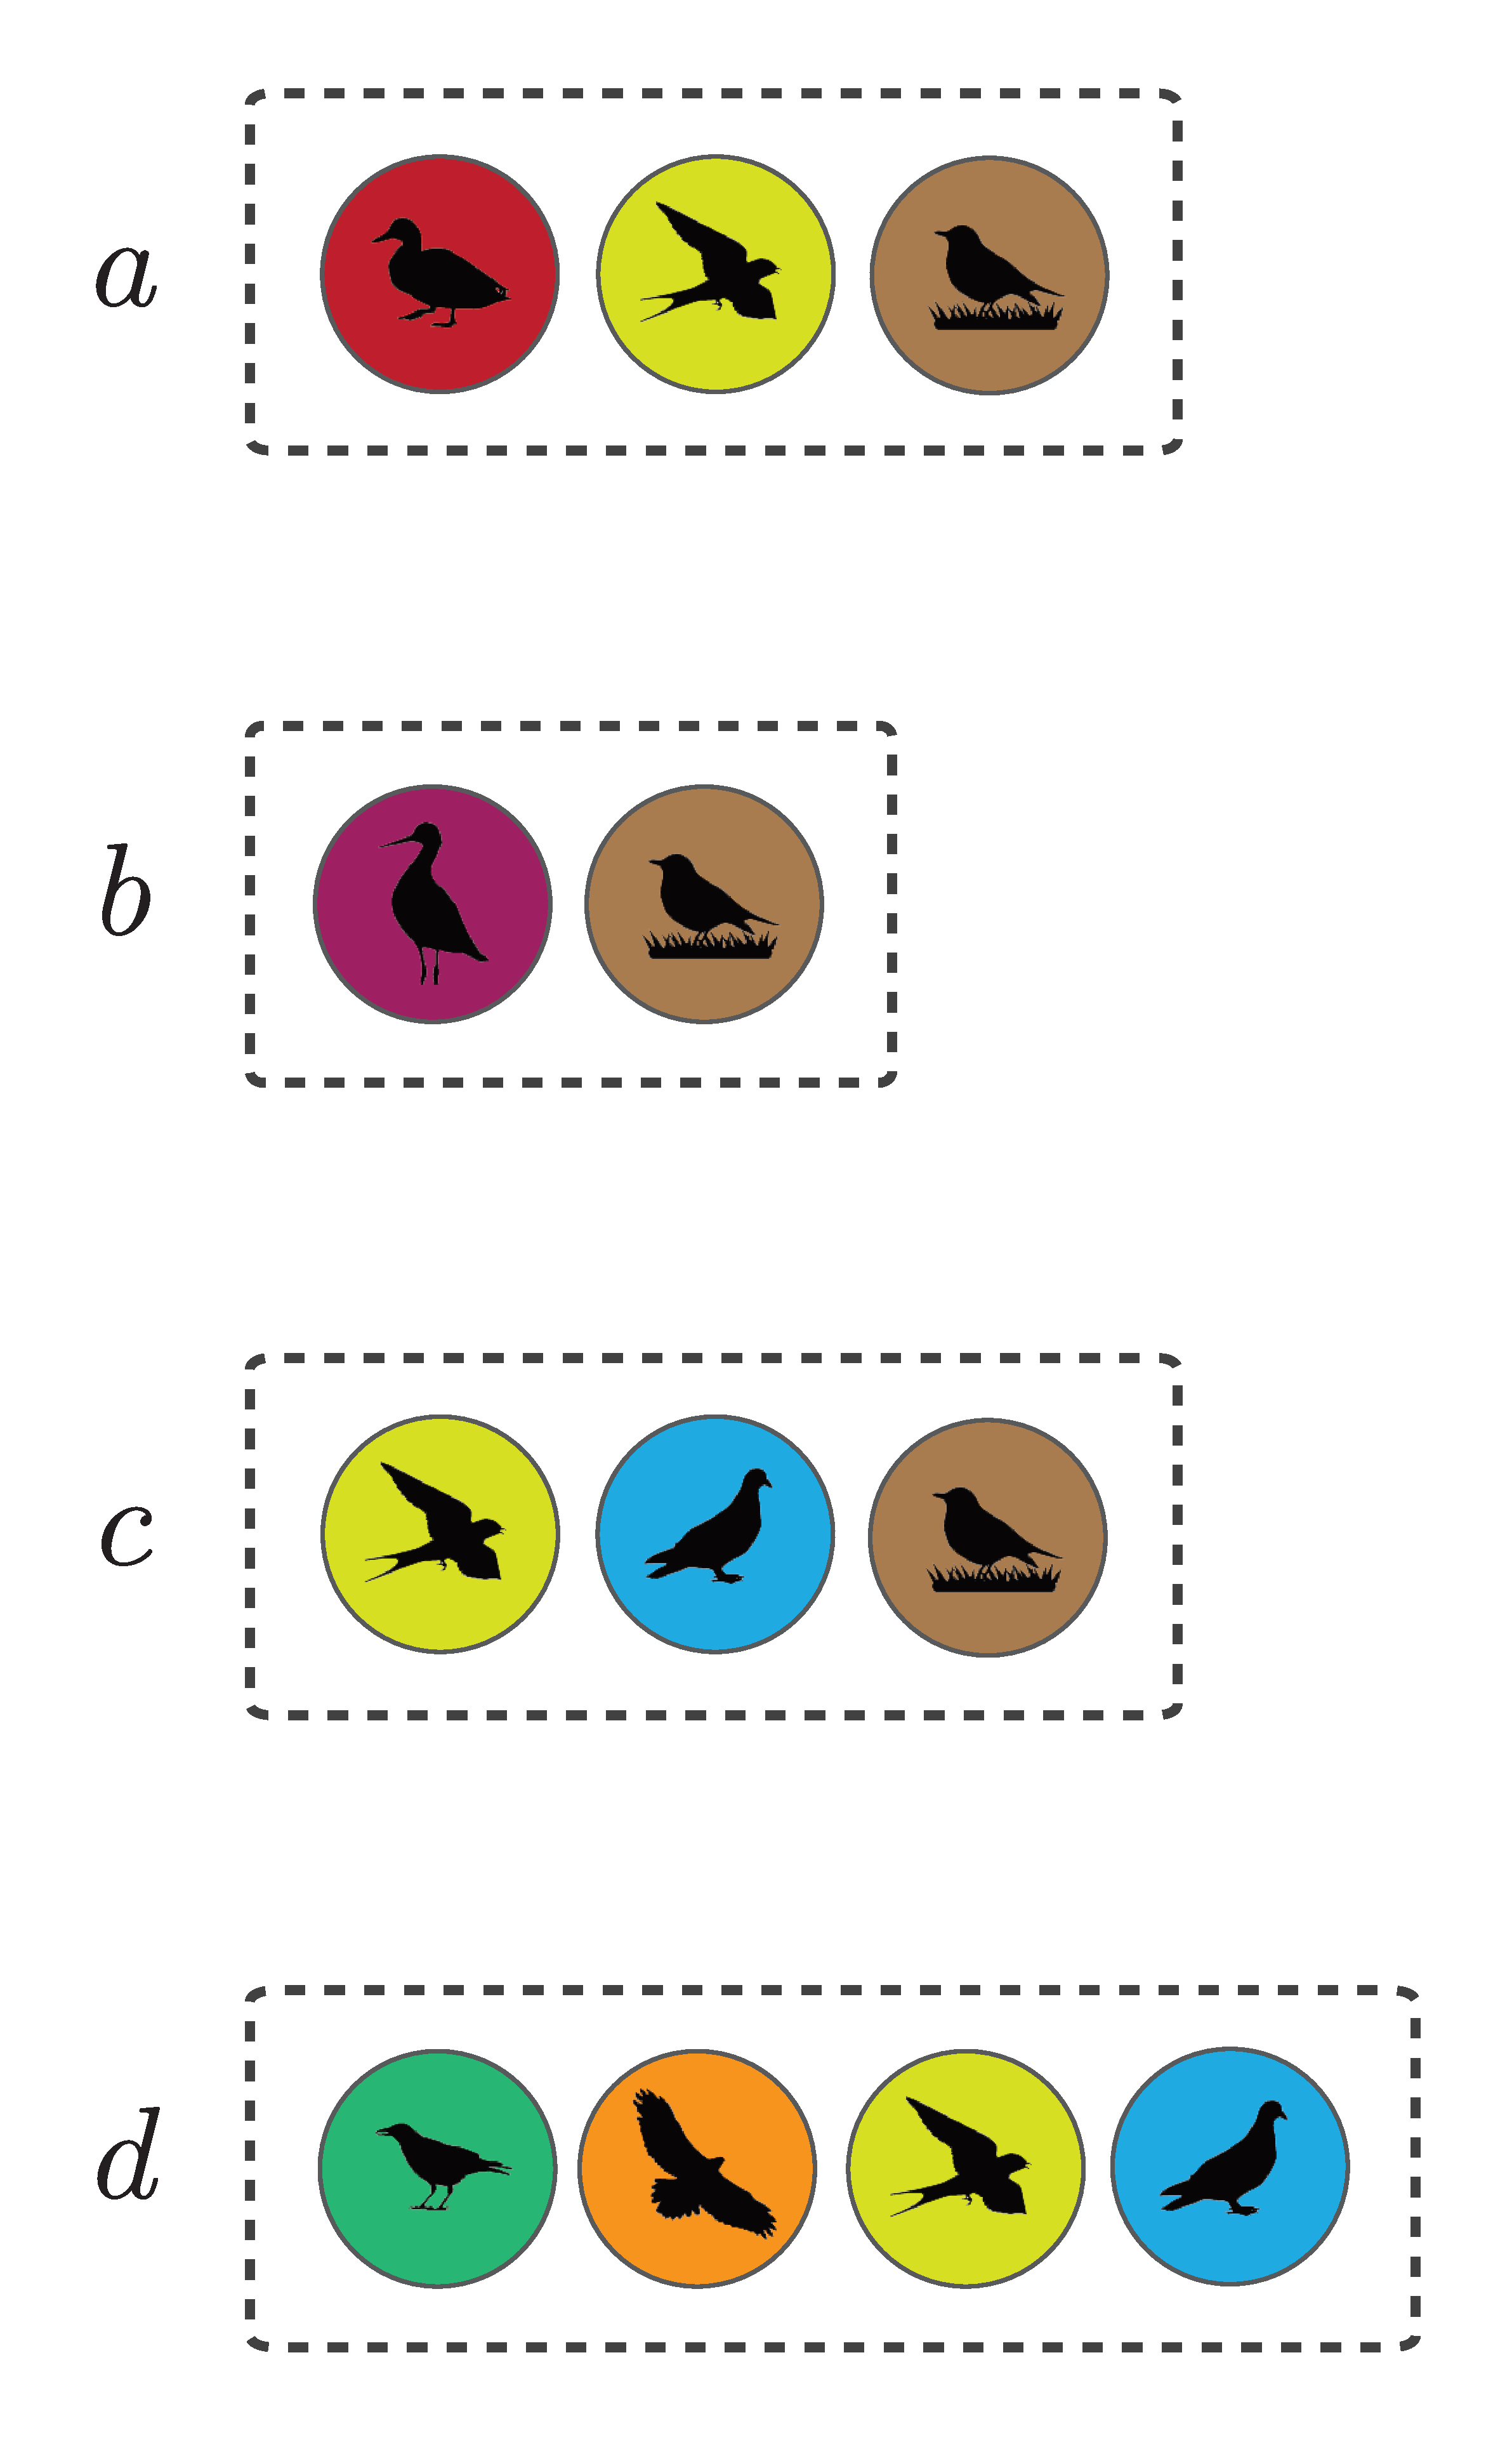
\includegraphics[width=2in]{figures/sets.pdf}
}
\end{columns}
\end{frame}

\begin{frame}{Greedy}

{\large Theorem} \qcite{Nemhauser et al., 1978}\\[1em]
\hspace{0.5em}If $f$ is monotone submodular, then greedy gives a (1 - 1/e)-approximation.
\end{frame}

\begin{frame}{Birdwatching with costs}
\centering
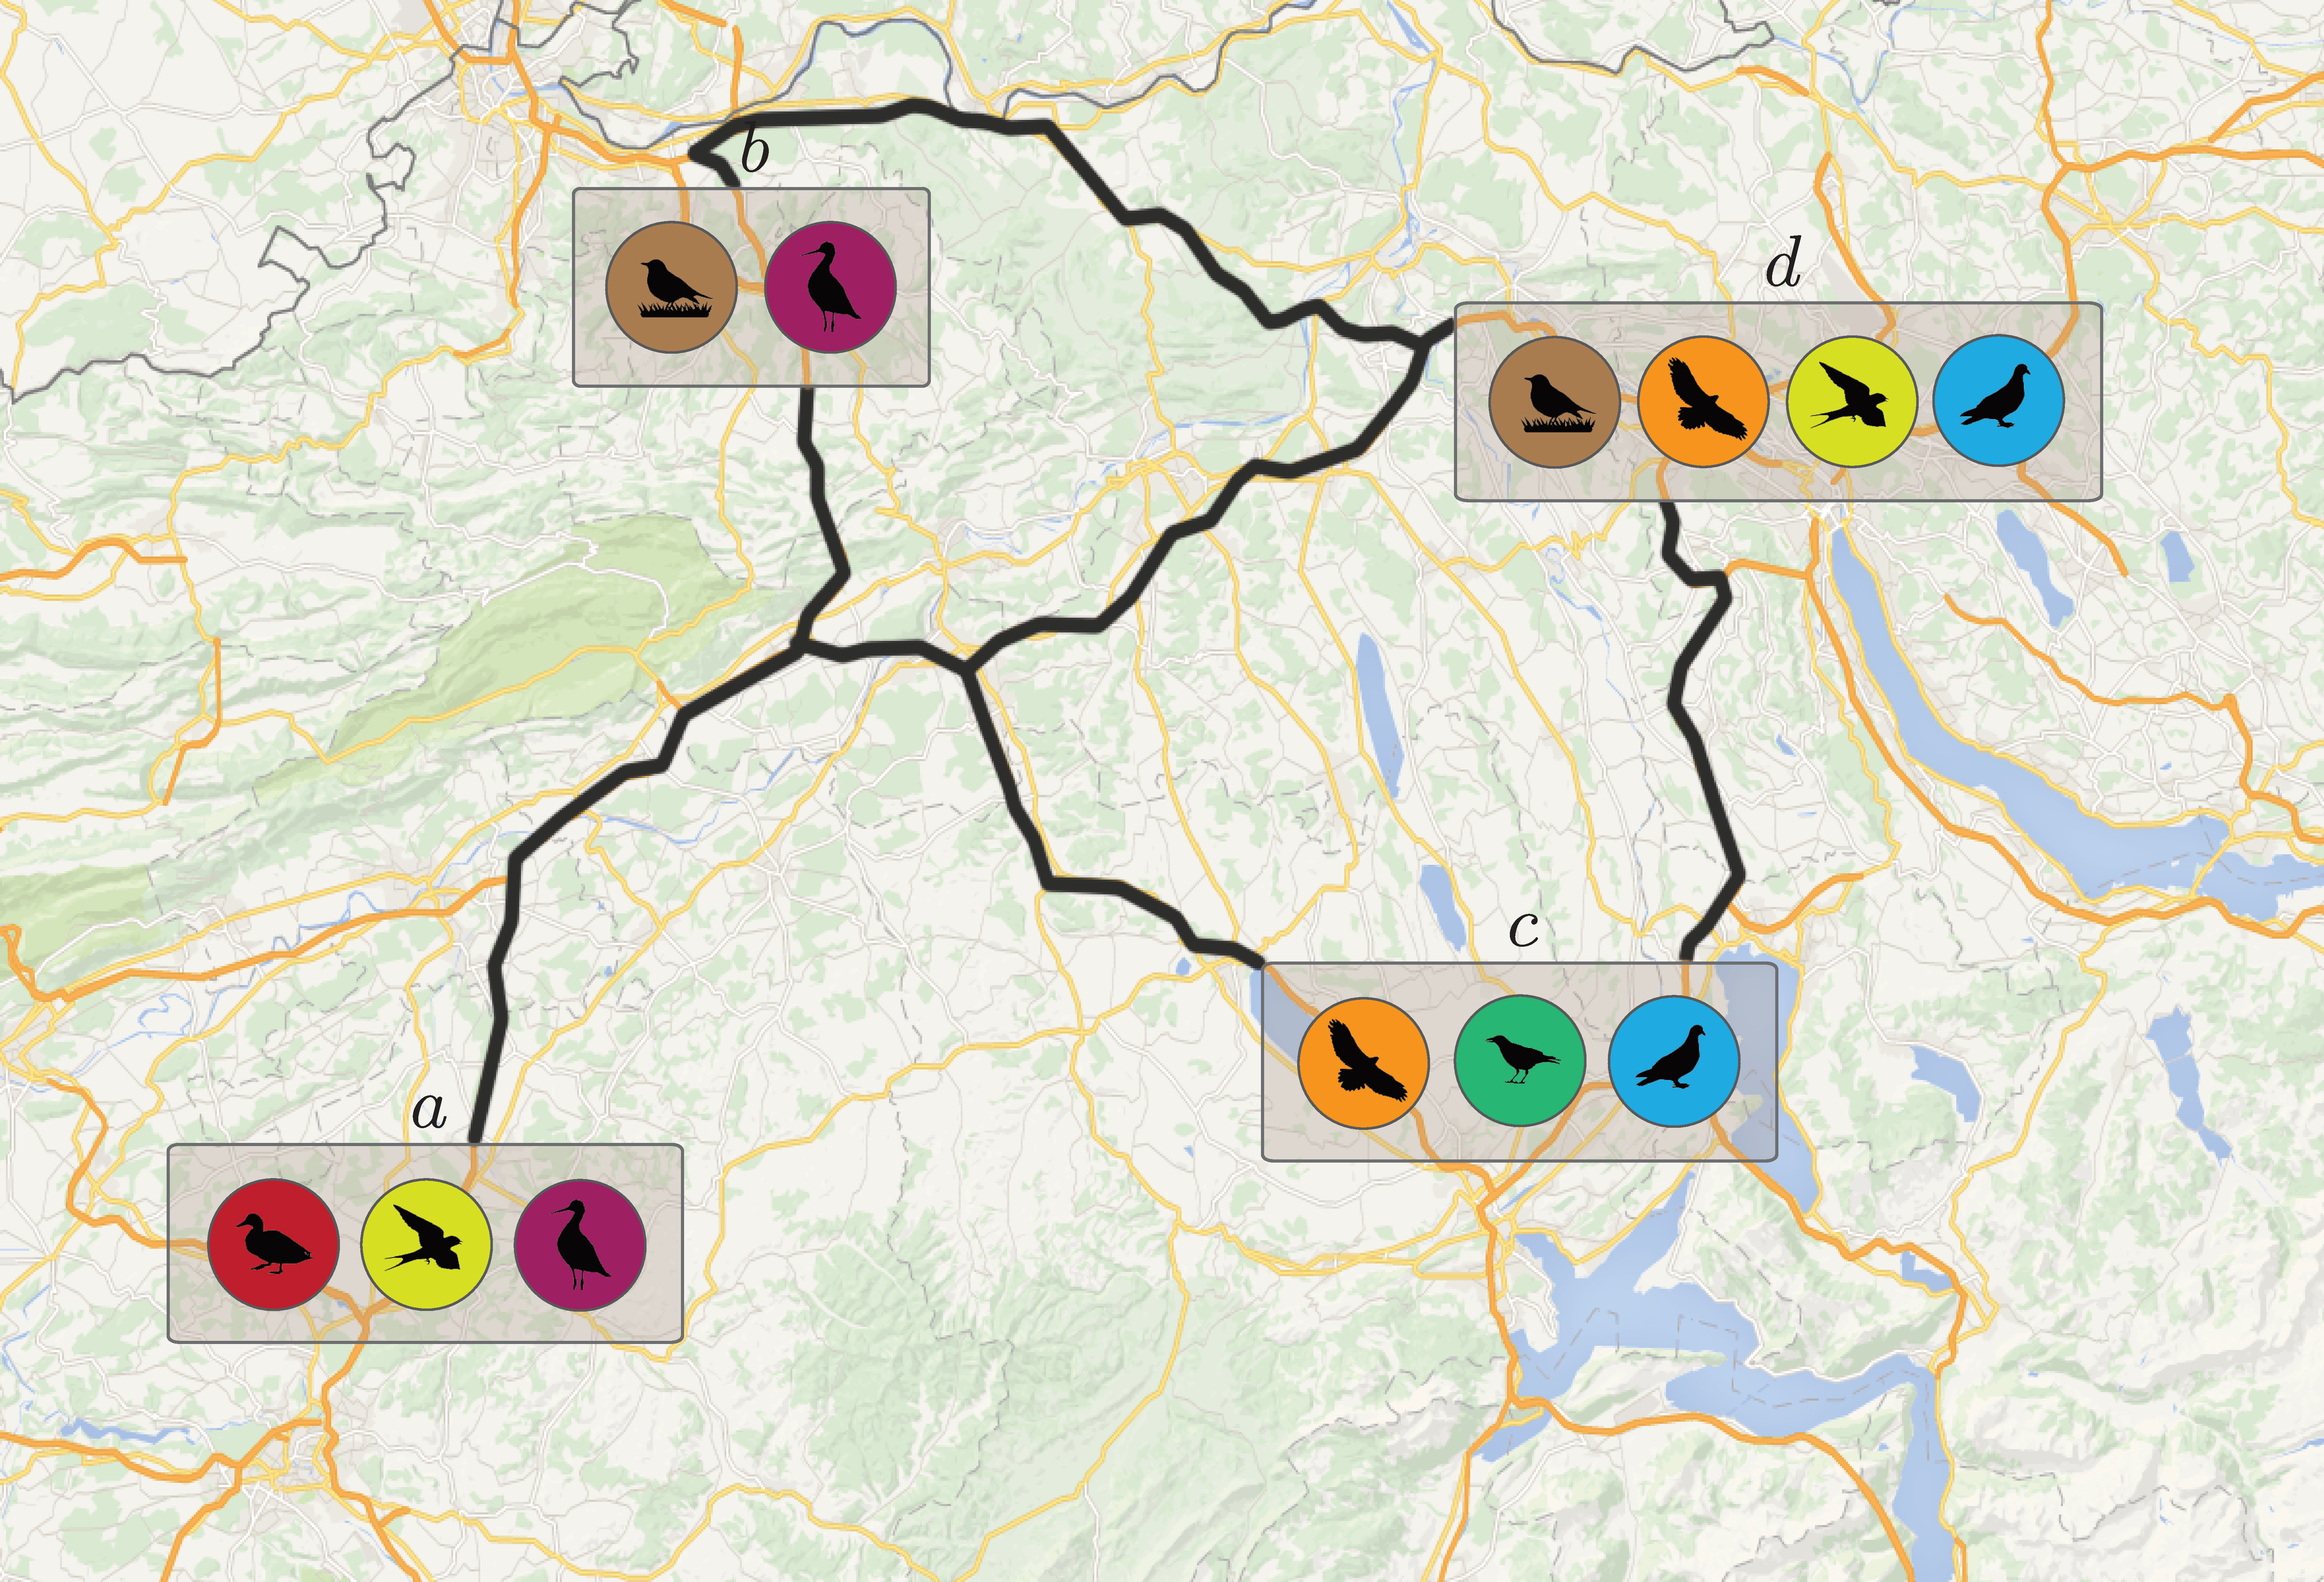
\includegraphics[width=4.75in]{figures/intro_roads.pdf}
\end{frame}

\end{document}
